%%%%%%%%%%%%%%%%%%%%%%%%%%%%%%%%%%%%%%%%%%%%%%%%%%%%%%%%%%%%%
%% HEADER
%%%%%%%%%%%%%%%%%%%%%%%%%%%%%%%%%%%%%%%%%%%%%%%%%%%%%%%%%%%%%
\documentclass[a4paper,twoside,10pt]{report}


%% Language %%%%%%%%%%%%%%%%%%%%%%%%%%%%%%%%%%%%%%%%%%%%%%%%%
\usepackage[USenglish]{babel} %francais, polish, spanish, ...
\usepackage[T1]{fontenc}
\usepackage[ansinew]{inputenc}

\usepackage{lmodern} %Type1-font for non-english texts and characters

\usepackage{hyperref}
\usepackage{enumerate}
\usepackage{caption}
\usepackage{subcaption}
\usepackage[sectionbib]{chapterbib}

%% Packages for Graphics & Figures %%%%%%%%%%%%%%%%%%%%%%%%%%
\usepackage{graphicx} %%For loading graphic files
%\usepackage{subfig} %%Subfigures inside a figure
%\usepackage{pst-all} %%PSTricks - not useable with pdfLaTeX


%% Math Packages %%%%%%%%%%%%%%%%%%%%%%%%%%%%%%%%%%%%%%%%%%%%
\usepackage{amsmath}
\usepackage{amsthm}
\usepackage{amsfonts}


%% Line Spacing %%%%%%%%%%%%%%%%%%%%%%%%%%%%%%%%%%%%%%%%%%%%%
%\usepackage{setspace}
%\singlespacing        %% 1-spacing (default)
%\onehalfspacing       %% 1,5-spacing
%\doublespacing        %% 2-spacing


%% Other Packages %%%%%%%%%%%%%%%%%%%%%%%%%%%%%%%%%%%%%%%%%%%
\usepackage{a4wide} %%Smaller margins = more text per page.
\usepackage{fancyhdr} %%Fancy headings
\usepackage{longtable} %%For tables, that exceed one page

%%%%%%%%%%%%%%%%%%%%%%%%%%%%%%%%%%%%%%%%%%%%%%%%%%%%%%%%%%%%%
%% DOCUMENT
%%%%%%%%%%%%%%%%%%%%%%%%%%%%%%%%%%%%%%%%%%%%%%%%%%%%%%%%%%%%%
\begin{document}

\pagestyle{empty} %No headings for the first pages.


%% Title Page %%%%%%%%%%%%%%%%%%%%%%%%%%%%%%%%%%%%%%%%%%%%%%%
%% ==> Write your text here or include other files.

%% The simple version:
\title{Distributed systems (H04I4A) - summary (version 1)}
\author{Joris Schelfaut}
%\date{} %%If commented, the current date is used.
\maketitle

%% The nice version:
%\input{titlepage} %%You need a file 'titlepage.tex' for this.
%% ==> TeXnicCenter supplies a possible titlepage file
%% ==> with its templates (File | New from Template...).

\chapter*{Foreword}

This is a summary for the course Gedistribueerde systemen\footnote{\url{http://onderwijsaanbod.kuleuven.be/syllabi/n/H04I4AN.htm}} given by Prof. Dr. Joosen\footnote{\url{https://distrinet.cs.kuleuven.be/people/wouter}} and Dr. Walraven\footnote{\url{https://distrinet.cs.kuleuven.be/people/showMember.do?memberID=u0059786}} at the Catholic University of Louvain\footnote{\url{http://www.kuleuven.be/english}} (KUL). The contents of this text are based on the book "Distributed Systems: Concepts and Design (5th Edition)"\footnote{\url{http://www.cdk5.net/wp/}} by Coulouris et al. and the lecture slides.

Note that this is not a complete summary and may become outdated as the contents of the course change over the years. I can also not guarantee that there are no errors in this text, so be aware of that. Other than that, feel free to use this text while studying the course.

This text is also available at \url{http://districted.wordpress.com/concepts/distributed-systems/}. The text on that website may be a bit more up-to-date, depending on how much work I'm willing to put into it. If there are any mistakes or you would like to give some feedback, feel free to let me know on that website.

Joris.

%% Inhaltsverzeichnis %%%%%%%%%%%%%%%%%%%%%%%%%%%%%%%%%%%%%%%
\tableofcontents %Table of contents
\cleardoublepage %The first chapter should start on an odd page.

\pagestyle{plain} %Now display headings: headings / fancy / ...



%% Chapters %%%%%%%%%%%%%%%%%%%%%%%%%%%%%%%%%%%%%%%%%%%%%%%%%
%% ==> Write your text here or include other files.

\part{Theory}
\chapter{Introduction}

A distributed system consists out of components that reside on different machines and communicate through message passing. This definition introduces three notable challenges:

\begin{enumerate}
	\item The lack of a global clock is largely resolved by coordinating actions through messages, but has its limitations.
	\item The nodes within this system may also fail independently and may even go undetected.
	\item Concurrency of operations brings another challenge as resources may be accessed simultanously, possibly introducing inconsistencies.
\end{enumerate}

Although these constraints make distributed systems complex to design, they come with significant benefits as well. The main motivation for developing and using distributed systems is resource sharing.

Middleware is the layer between architecture and application. It introduces an abstraction layer to build distributed applications, hiding the heterogeneity of the underlying architectural elements, e.g. protocols, servers, operating systems and so on. Middleware technology may be provide certain services such as distribution, security, ... [1]

\section*{Overview}

The following topics are addressed in this text:

\begin{itemize}
	\item \textbf{Direct communication} : This article discusses protocols and paradigms for direct communication in distributed systems such as remote procedure call and remote method invocation.
	\item \textbf{Indirect communication} : This article discusses protocols and paradigms for indirect communication in distributed systems such as group communication, message queues and publish-subscribe systems.
	\item \textbf{Distributed file systems} : This article gives an introduction to distributed file systems such as Sun NFS and the Andrew File System.
	\item \textbf{Distributed transactions} : This article gives an overview of some concepts related to distributed transactions such as distributed deadlock and commit protocols.
	\item \textbf{Replication} : This article explains the basics of replication and gives an overview of the Coda file system.
	\item \textbf{Cloud computing} : Introduction to cloud computing.
\end{itemize}


\section*{References}

\begin{itemize}
	\item [1] G. Coulouris, J. Dollimore, T. Kindberg and G. Blair, "Distributed Systems: Concepts and Design (5th Edition)", M. Horton, Red., Addison-Wesley, 2011, p. 1063.
\end{itemize}



\section*{Links}

\begin{itemize}
	\item http://docs.oracle.com/javase/7/docs/technotes/guides/rmi/ : Java RMI overview by Oracle;
	\item http://docs.oracle.com/javaee/5/tutorial/doc/docinfo.html : JEE tutorial by Oracle;
	\item https://developers.google.com/appengine/docs/java/ : Google App Engine Java overview.
\end{itemize}
\chapter{Direct communication}

\section{Introduction}


\subsection{Data representation}

\emph{Marshalling} is the assembling of a collection of data items into a form suitable for transmission, whereas \emph{unmarshalling} is the disassembling of a message on arrival to produce the equivalent collection of data items. For example Java uses serialization and deserialization of objects, or SOAP in Service Oriented Architectures et cetera [2].


\subsection{Message passing}

\textbf{Table 1} lists the two basic operations in message passing.

\begin{table}
	\caption{Basic message passing API.}
	\label{tab:}
	\begin{tabular}{p{150px} | p{250px}}
		\textbf{Operation} & \textbf{Description} \\
		\hline
		send (p: PortId; m: Message) & Send a message \emph{Message} to a process at a port with given \emph{PortId}. \\
		receive (p: PortId; VAR m: Message) & Receive a message \emph{Message} while listening at a port with given \emph{PortId}. \\
		\hline
	\end{tabular}
\end{table}


The semantics of send and receive operations can differ. In \emph{synchronous} send the process waits for the corresponding receive. In synchronous receive, the process waits for the message arrival. In \emph{asynchronous} send the process does not wait for the message arrival. In aynschronous receive, the process announces its willingness to accept or check for message arrival [2].

There a various possible message destinations, e.g., \emph{processes}, which have a single entry point per process for all messages, or \emph{ports}, which have one receiver and possibly many senders, or \emph{mailboxes}, which may have many receivers [2].


\subsubsection{Reliable communication}

Failures in message passing may be the result of a number of causes, for example corrupted messages, duplicate messages, omission, i.e., the loss of messages, wrong ordering of messages, or receiver process failures [2]. In order to achieve reliable communication, messages should be delivered uncorrupted, in order, without duplicates, despite a reasonable number of packets dropped or lost. Unfortunately perfectly reliable communication can not often be guaranteed [2].

Reliable communication can be implemented using a number of techniques, for example [2]:
\begin{itemize}
	\item \textbf{Corruption} : Include checksum in message;
	\item \textbf{Order mistakes and duplicates} : Include a message number which identifies the message;
	\item \textbf{Omission} : Sender stores message in buffer, sends it and sets a time-out and the receiver replies with acknowledgement. If no aknowledgement was received, the sender retransmits messages after timeout.
\end{itemize}



\section{Remote invocation}

\subsection{Request-reply protocols}

Request-reply protocols are designed to support roles and message exchanges in typical client-server interactions. \textbf{Table 2} lists the basic operations of request-reply protocols. \textbf{Figure 1} shows the general model for request-reply protocols.


\begin{table}
	\caption{Basic request-reply protocol operations.}
	\label{tab:}
	\begin{tabular}{p{150px} | p{250px}}
		\textbf{Operation} & \textbf{Description} \\
		\hline
		doOperation		& The client sends request and returns answer to the application program. \\
		getRequest		& The server gets the request from the client. \\
		sendReply			& The server sends a reply to the client. \\
		\hline
	\end{tabular}
\end{table}


\begin{figure}
	\begin{center}
		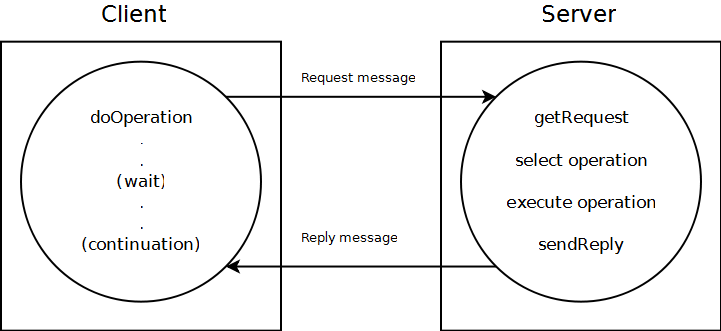
\includegraphics[width=0.7\textwidth]{img/requestreplycommunication}
	\end{center}
	\caption{Model for request-reply communication.}
	\label{fig:requestreplycommunication}
\end{figure}



\subsubsection{Reliable communication}

In reliability measures of TCP are an overkill as the acknowledgement from the receiver is redundant because the reply message is an acknowledgement. As a result, UDP can be used for building more efficient client server communication [2].



\subsection{Remote procedure call}

Traditional applications consist of a main program with a number of procedures (functions). In distributed systems procedures are grouped into servers, and main programs become clients. To achieve transparency the (remote) operations on a server from a client should look like conventional procedure calls [2].

To achieve this an additional message subsystem is introduced. When an application program calls client \emph{stub procedure}, the client stub procedure marshalls parameters of call and gives it to \emph{communication module} in client. The communication module then transmits a message with the marshalled RPC to the server's communication module who passes it on to the \emph{dispatcher}. The dispatcher determines which procedure is called and calls the correct server stub procedure. Next, the server stub procedure unmarshalls data and calls the relevant server procedure. The server procedure returns the answer to the server stub procedure. The result is marshalled and sent to the client via the communication modules. The communication module at client side gives data to client stub procedure, who finally unmarshalls data and returns the answer to the calling program [2]. \textbf{Figure 2} shows the architectural elements in this scenario.


\begin{figure}
	\begin{center}
		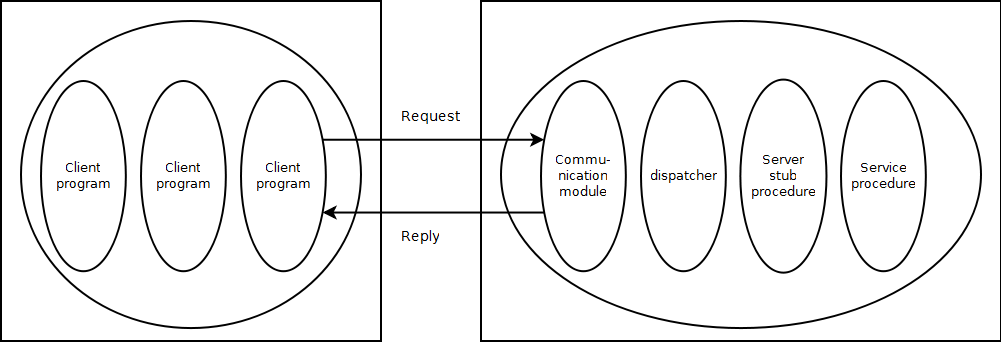
\includegraphics[width=0.7\textwidth]{img/rpc}
	\end{center}
	\caption{Remote procedure call.}
	\label{fig:rpc}
\end{figure}

\emph{Remote procedure calls} (RPC) can be integrated within a particular programming language, or based on a special \emph{interface definition language} (IDL) [2].


\subsubsection{Design issues}

\paragraph{Heterogeous environment}

An Interface Definition Language (IDL) tries to provide abstraction for the heterogeneity of client and server implementations through programming language-independency. IDL describes operation signatures and its interface compilers are used as a base for generating client and server stubs, which can be implemented in different languages [2].


\paragraph{Transparancy}

To achieve transparency, RPC should be as much like local procedure calls as possible. However the calling instruction set is different, and there is no shared memory between caller and callee [2].

RPC requires some form of exception handling as failures cannot be hidden. Clients cannot distinguish between network failures or server failures. To deal with failures, language specific solutions may be applied, expressive return codes of functions, or extensions provided by IDL [2].

\paragraph{Semantics}


Remote procedure calls may have the following semantics [2]:
\begin{itemize}
	\item \textbf{Maybe} : Requests are not resent, as a result no duplicate filtering is required, and it logically follows that procedure need no re-exececution, and no replies are re-transmited;
	\item \textbf{At-least-once} : Requests are re-sent, but as there is no duplicate filtering, procedures can be re-exececuted. To retain system consistency, operations have to be idempotent;
	\item \textbf{At-most-once} : Requests are re-sent, hence duplicate filtering is required and replies are re-transmitted. Procedures can not be re-exececuted;
	\item \textbf{Exactly-once} : Difficult or impossible given failures;
\end{itemize}



\subsubsection{Implementation aspects}

The task of the interface compiler is to generate client and server stub procedures, marshalling and unmarshalling operations for each argument type, and implement headers for server procedures.

Binding is the linking of the client to the server at execution time: the server will register a service at binder, and the client will perform a lookup for the service. Locating the binder is done through a well-known host address and is the responsibility of the operating system [2].


\subsubsection{Asynchronous RPC}

Asynchronous RPC can be used to reduce the idle time of processes that are waiting for a remote procedure call to complete [2].



\subsubsection{Conclusions}

RPC is a familiar paradigm which has been a basic primitive for distributed programming for many applications and systems [2].

RPC has some limitations with respect to failure handling, no transaction support, and the fact that RPC only supports one-to-one communication [2].



\subsection{Remote method invocation}

\emph{Remote method invocation} (RMI) is a technology that similar to RPC allows clients to invoke methods on remote objects. It also uses programming with interfaces, called \emph{remote interfaces}, can offer a number of call semantics and provides a similar level of transparancy as RPC, i.e., local and remote calls have the same syntax but the distributed nature of calls can be exposed, e.g., through remote exceptions. As a result, they share many of the design issues explained earlier, with the additional design issue of dealing with (distributed) objects for RMI [1].

RMI allows parameter passing by value, as input or output parameters, and also as object references. Remote invocation can then be used on these object references, instead of transmitting the complete object value accross the network [1]. The possible remote invocations are listed in the remote interface of that object.


\subsubsection{Distributed objects}

\paragraph{Classic object model}

Objects are accessed via their reference. An object is associated with an interface, which separates the method signatures from the actual implementation. Actions in object-oriented programs are initiated by invoking a method in another object [1]. Three possible effects are associated with method invocation [1]:
\begin{enumerate}
	\item Change of the target object state, which consists of the values of its instance variables;
	\item Creation of a new object;
	\item Resulting in a new invocation on methods in other objects.
\end{enumerate}
To deal with errors during execution, exceptions are used to create clearer error handling in complex code. Exceptions are a way to alter the control flow of a program [1].

A garbage collector detects when objects are no longer used and frees the memory occupied by these instances.

\paragraph{Distributed object model}

\emph{Distributed objects} are objects that are managed by a server and implement a \emph{remote interface} by which clients can invoke on the distributed object via its \emph{remote object reference}. A remote object reference is an identifier that can be used throughout the distributed system to refer to a unique remote object [1].

\emph{Remote exceptions} reveal some of distributed nature of RMI. Aside from errors in the program, exceptions in remote objects may be due to crashes in the server process, timeouts due to network failure et cetera [1].

In a distributed context, distributed garbage collection is slightly more complicated as object references may be spread accross different machines. It is achieved by extending the local garbage collection with a distributed module, often based on reference counting [1].


\subsubsection{RMI implementation}

\textbf{Figure 3} shows the remote method invocation architectural components. In what follows we describe some of these components in more detail to finally form the complete picture of the RMI technology.

\begin{figure}
	\begin{center}
		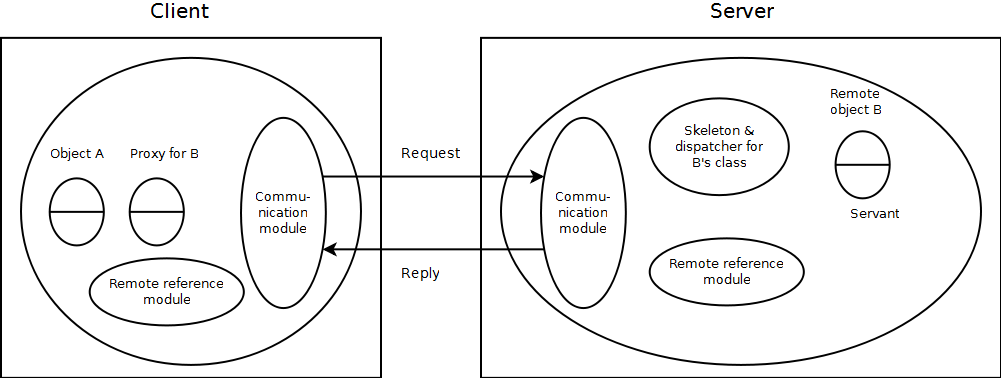
\includegraphics[width=0.7\textwidth]{img/rmi}
	\end{center}
	\caption{Remote method invocation.}
	\label{fig:rmi}
\end{figure}


\paragraph{Communication module}

Communication modules operate using a request-reply protocol between client and server. They are responsible for enforcing specific invocation semantics, e.g., \textit{at-most-once} [1].

When a request is received by the server's communication module, the communication module passes on the remote reference in the request to the remote reference module which returns the local reference. Next the server's communication module selects the dispatcher for the class of the object to be invoked (cf. RPC), passing on the local reference [1].


\paragraph{Remote reference module}

The task of the \emph{remote reference module} is to translate between remote and local references by looking them up in a \emph{remote object table}. The remote object table holds the following information [1]:
\begin{itemize}
	\item Each remote object held by the process at the server's remote reference module;
	\item Each local proxy at the client's remote reference module.
\end{itemize}


\paragraph{RMI software layer}

The \emph{RMI software layer} is a layer between the application-level objects and the communication and remote reference modules. The following middleware components are part of this layer [1]:

\begin{itemize}
	\item \textbf{Proxy} : The proxy appears as a normal object in the client process, achieving some transparancy. However, instead of executing invocations, it forwards them in a message to the corresponding remote object after marshalling arguments. Results from the invocation are then unmarshalled and passed on to the client process;
	\item \textbf{Dispatcher} : For each class representing a remote object there is one skeleton and one dispatcher at the server. The dispatcher receives requests from the communication module;
	\item \textbf{Skeleton} : The class of a remote object has a skeleton, which implements the methods in the remote interface. It is responsible for marshalling and unmarshalling arguments and results respectively of requests before passing them on to the servant. A \emph{servant} is an instance of a class that provides the body to a remote object. Servants live within a server process and handles the remote requests passed on by the corresponding skeleton;
\end{itemize}




\section*{References}

\begin{enumerate}[1]
	\item G. Coulouris, J. Dollimore, T. Kindberg and G. Blair, "Distributed Systems: Concepts and Design (5th Edition)", M. Horton, Red., Addison-Wesley, 2011, p. 1063.
	\item W. Joosen, 2013, "Distributed Systems Direct Communication PART I", iMinds-DistriNet, KULeuven
	\item W. Joosen, 2013, "Distributed Systems Direct Communication PART II", iMinds-DistriNet, KULeuven
\end{enumerate}
\chapter{Indirect communication}


\section{Introduction}

In [1] \emph{indirect communication} is defined as "communication between entities in a distributed system through an intermediary with no direct coupling between sender and receiver". Uncoupling may be established in two ways:

\begin{itemize}
	\item \textbf{Space} : The sender does not (need to) know the identity of the receiver.
	\item \textbf{Time} : The sender and receiver does not (need to) exist at the same time as the receiver.
\end{itemize}

\textbf{Table 1} categorizes a number of technologies according to their support for time and/or space uncoupling. Note the relationship between time uncoupling and asynchronous communication. However, in the case of strict uncoupling in time, the receiving end does not necessarily exist at the time of sending, as mentioned earlier [1].


\begin{table}
	\caption{Overview of space and time coupling for distributed communication paradigms.}
	\label{tab:}
	\begin{tabular}{p{100px} | p{125px} | p{125px}}
															& \textbf{Time-coupled} 	& \textbf{Time-uncoupled} \\
		\hline
		\textbf{Space-coupled} 		& Message-passing, RMI 		&  \\
		\textbf{Space-uncoupled} 	& IP multicast						& Publish-subscribe, tuple spaces, message queues \\
		\hline
	\end{tabular}
\end{table}

Typical applications of indirect communication is in mobile environments, cloud computing, and event dissemination where receivers are unknown or change rapidly [1].



\section{Paradigms}

\subsection{Group communication}

In group communication the messages within a distributed system are sent to a group, and from there sent to all other members of the group. The sender has no knowledge of the identities of the receivers, hence the indirection [1]. This kind of communication is called broadcasting where the sender forms a one-to-many relationship with the other members of the group.

Groups may be open or closed. In closed groups only members can multicast to it, opposed to open groups where processes outside the group can multicast to it as well.

\textbf{Figure 1} gives an overview of the basic operations of group management. The operation set for group communication is shown in \textbf{table 2}.


\begin{figure}
	\begin{center}
		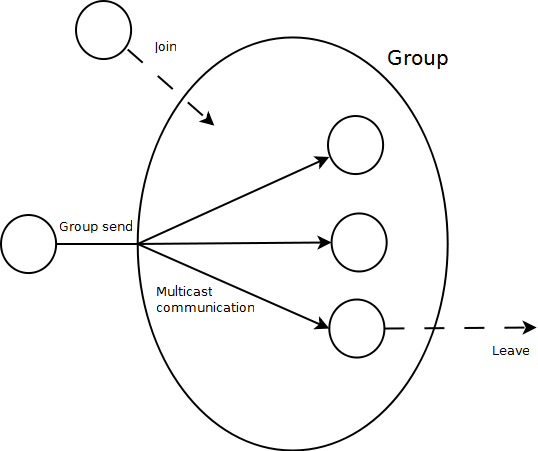
\includegraphics[width=0.5\textwidth]{img/groupcommunication}
	\end{center}
	\caption{Group membership management in group communication.}
	\label{fig:groupcommunication}
\end{figure}

\begin{table}
	\caption{Group communication API.}
	\label{tab:api:groupcommunication}
	\begin{tabular}{p{150px} | p{250px}}
		\textbf{Operation} & \textbf{Description} \\
		\hline
		join (group) & \emph{A process joins the group.} \\
		leave (group) & \emph{A process leaves the group.} \\
		send (group, message) & \emph{Send a message to the group. The group indirection layer propagates the message to all other members.} \\
		\hline
	\end{tabular}
\end{table}


\subsection{Publish-subscribe systems}

A publish-subscribe system is a platform where \emph{subscribers} can subscribe to certain events provides by \emph{publishers}. The system then matches published events against subscriptions. Subscribers then receive an update if successful matches are found.

Publishers form a one-to-many relationship with their subscribers, but the publishers do not know who is subscribed. Subscribers also do not need to know the publisher, as long as they can specify which kind of messages they would like to receive . Publish-subscribe systems are uncoupled in time as they provide asynchronous communication between senders and receivers [1].

The operations of a publish-subscribe system are listed in \textbf{Table 3}.


\begin{table}
	\caption{Publish-subscribe system API.}
	\label{tab:api:publishsubscribersystems}
	\begin{tabular}{p{150px} | p{250px}}
		\textbf{Operation} & \textbf{Description} \\
		\hline
		publish (event) 			& \emph{A publisher publishes an event.} \\
		subscribe (filter) 		& \emph{A subscriber subscribes to a set of events through a filter.} \\
		unsubscribe (filter) 	& \emph{A subscriber unsubscribes from a set of events.} \\
		notify (event) 				& \emph{Deliver events to its subscribers.} \\
	  advertise (filter) 		& \emph{A publisher declare the nature of the events they will produce.} \\
		unadvertise (filter) 	& \emph{A publisher revokes the advertisement.} \\
		\hline
	\end{tabular}
\end{table}



\begin{figure}
	\begin{center}
		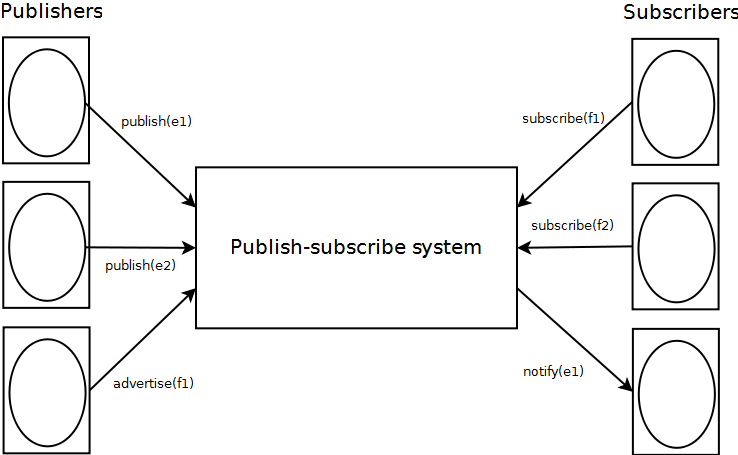
\includegraphics[width=0.6\textwidth]{img/publish-subscribesystem}
	\end{center}
	\caption{Publish-subscribe system architecture.}
	\label{fig:publish-subscribesystem}
\end{figure}




\subsection{Message queues}

Message queues are a form of message-oriented middleware. A message queue introduces a layer of indirection between \emph{producers} and \emph{consumers}. A producers sends messages to a queue, next consumers receive messages from these queues. Message queues are uncoupled in time, but not in space. The relation between a consumer and a producer through a message is one-to-one [1].

The operations that can be invoked on a message queue are listed in \textbf{table 4}.


\begin{table}
	\caption{Message queue API.}
	\label{tab:api:messagequeues}
	\begin{tabular}{p{150px} | p{250px}}
		\textbf{Operation} & \textbf{Description} \\
		\hline
		send (message) & \emph{A producer sends a message to the queue.} \\
		receive (message) & \emph{A blocking receive operation. The consumer will block until an appropriate message is available.} \\
		poll (message) & \emph{The consumer checks the status of the queue. A message is returned if available, else a negative signal.} \\
		notify (message) & \emph{Start listening for event notications if a message is available.} \\
		\hline
	\end{tabular}
\end{table}


Messages are usually added to the queue based on the first-in-first-out (FIFO) policy, but priorities may be used as well. Message queues try to ensure reliable delivery by persisting messages: messages are eventually delivered (time uncoupling). Messages are also only sent once and as received to provide integrity [1].

The consumers may receive messages by actively checking (polling) if messages are available, or by receiving notifications that messages have become available. Messages may be filtered based on certain properties [1].

\begin{figure}
	\begin{center}
		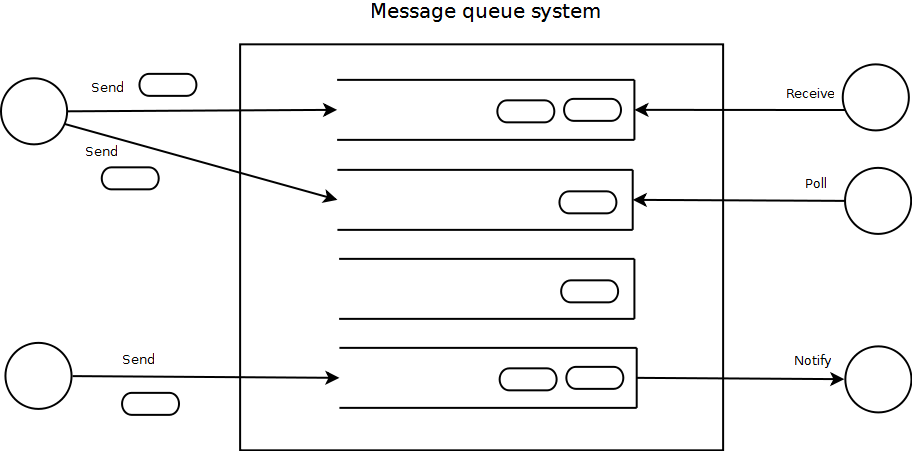
\includegraphics[width=0.7\textwidth]{img/messagequeues}
	\end{center}
	\caption{The message queue paradigm.}
	\label{fig:messagequeues}
\end{figure}



\subsection{Distributed shared memory}

The objective of distributed shared memory (DSM) is to share data between computers. Each computer has a local copy of the data. This data is kept up to date by passing messages between each node over the DSM middleware. \textbf{Table 5} shows the operations for DSM.

\begin{table}
	\caption{Distributed shared memory API.}
	\label{tab:api:dsm}
	\begin{tabular}{p{150px} | p{250px}}
		\textbf{Operation} & \textbf{Description} \\
		\hline
		read (data) 			& \emph{Read from the shared memory.} \\
		write (data) 			& \emph{Write to the shared memory} \\
		update (message) 	& \emph{Send an update message to the other members of the distributed shared memory.} \\
		\hline
	\end{tabular}
\end{table}


\begin{figure}
	\begin{center}
		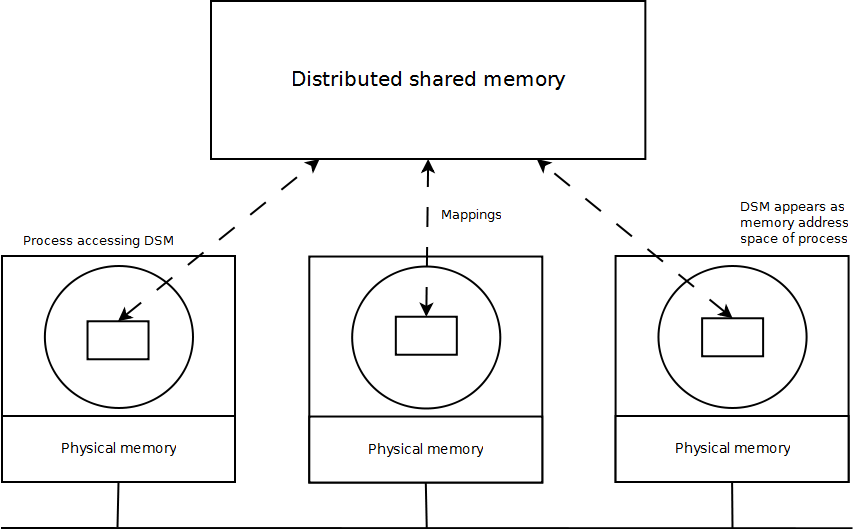
\includegraphics[width=0.6\textwidth]{img/dsm}
	\end{center}
	\caption{Distributed shared memory architecture.}
	\label{fig:dsm}
\end{figure}



\subsection{Tuple spaces}

A tuple space is a form of distributed memory where "processes communicate indirectly by placing tuples in a tuple space from which other processes can read and remove them" [1]. Space uncoupling is achieved as the sending and receiving processes may come from anywhere. Tuples may be taken from the space at any time and may even reside indefinately in the tuple space, thus achieving time uncoupling.

A tuple is typically of the form <var1, var2>, e.g. \emph{<"hugo",1.19>}. A number of operations can be executed on a tuple space as listed in \textbf{table 6}.


\begin{table}
	\caption{Tuple space API.}
	\label{tab:api:tuplespaces}
	\begin{tabular}{p{150px} | p{250px}}
		\textbf{Operation} & \textbf{Description} \\
		\hline
		read (tuple) 	& \emph{Reads a tuple from the tuple space.} \\
		take (tuple) 	& \emph{Extract a tuple from the tuple space.} \\
		write (tuple) & \emph{Write a new tuple to the tuple space.} \\
		\hline
	\end{tabular}
\end{table}


\begin{figure}
	\begin{center}
		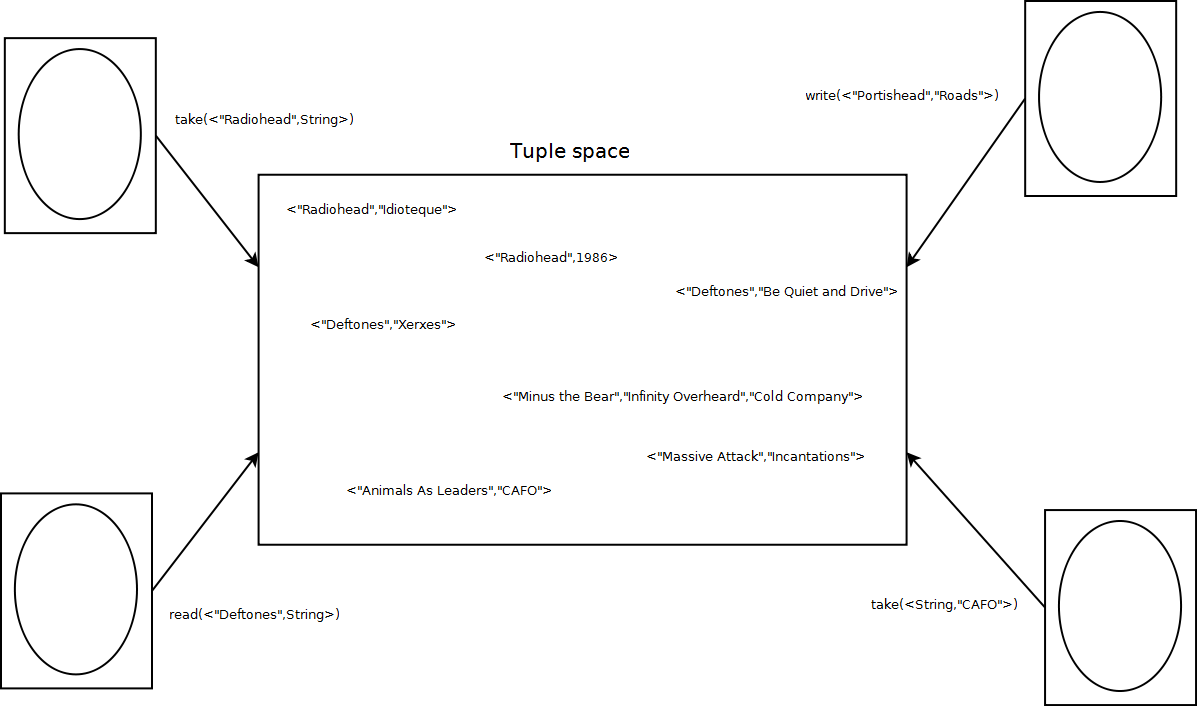
\includegraphics[width=0.6\textwidth]{img/tuplespace}
	\end{center}
	\caption{Tuple space abstract example.}
	\label{fig:tuplespace}
\end{figure}




\section*{References}

\begin{enumerate}[1]
	\item G. Coulouris, J. Dollimore, T. Kindberg and G. Blair, "Distributed Systems: Concepts and Design (5th Edition)", M. Horton, Red., Addison-Wesley, 2011, p. 1063.
\end{enumerate}
\chapter{Distributed file systems}


\section{Definitions, architectural model and requirements}

A distributed file system enables persistent data storage throughout an intranet. The objective of a distributed file service is resource sharing in an effort to reduce costs of storage and data management. Examples of these file systems are \emph{Sun NFS} and the \emph{Andrew File System (AFS)}, which will be discussed later.

\emph{Files} form an elementary unit of a file system. A file consists of the actual data and a number of attributes, e.g. file length and timestamp. File naming is determined in \emph{directories} in which text names are mapped to file identifiers. Files can be managed and manipulated through a series of operations such as create, read and write.


\subsection{Design requirements}

When designing a distributed file system, a number of transparency requirements should be taken into account. For example: \emph{access transparency}, i.e., the set of operations for both local and remote files is the same, \emph{location transparency}, i.e., the representation of the file system does not reveal the physical location of the files, or \emph{mobility transparency}, i.e., when files are moved, no client code or administration tables should be altered.

Other requirements are for example maintaining file consistency, security (e.g. through Access Control Lists), concurrent file updates, replication and fault tolerance.


\subsection{Architectural model design}

The following architectural model is based on the implementation of both NFS and AFS. It considers three separate modules dividing responsibilities between them [1]:

\begin{itemize}
	\item \textbf{Flat file service} : Provides an implementation for operations on the file contents. \emph{Unique file identifiers (UFID)} are used to refer to files in all flat file service operations.
	\item \textbf{Directory service} : Provides a mapping between text names for files and their UFIDs and operations on directories.
	\item \textbf{Client module} : Provides a single programming interface for the flat file service and directory service and runs on a each client machine.
\end{itemize}

\textbf{Figure 1} gives a schematic overview of this model.


\begin{figure}
	\begin{center}
		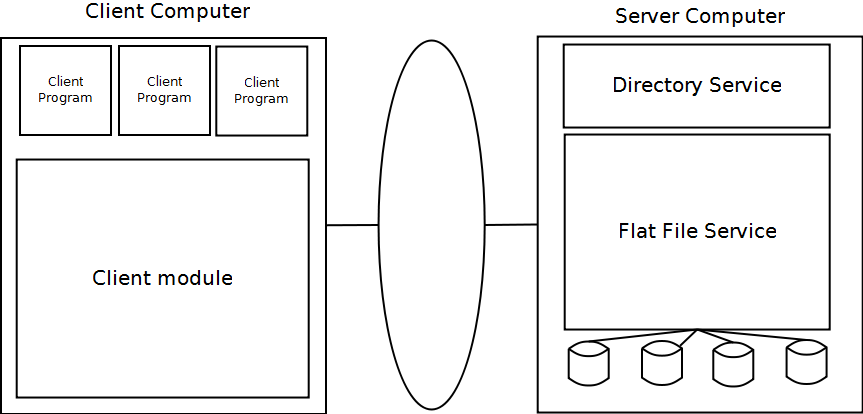
\includegraphics[width=0.7\textwidth]{img/fileservicearchitecture}
	\end{center}
	\caption{File service architecture.}
	\label{fig:fileservicearchitecture}
\end{figure}


\begin{table}
	\caption{Flat file system API, adapted from [1].}
	\label{tab:api:flatfilesystem}
	\begin{tabular}{p{150px} | p{250px}}
		\textbf{Operation} & \textbf{Description} \\
		\hline
		Read(FileId, i, n) $\rightarrow$ Data - throws BadPosition 	& \emph{If $1 \leq i \leq Length(File)$ : Reads a sequence of up to n items from a file starting at item i and returns it in Data.} \\
		Write(FileId, i, Data) - throws BadPosition 						& \emph{If $1 \leq i \leq Length(File)+1$ : Writes a sequence of Data to a file, starting at item i, extending the file if necessary.} \\
		Create() $\rightarrow$ FileId 																& \emph{Creates a new file of length 0 and delivers a UFID for it.} \\
		Delete(FileId) 																					& \emph{Removes the file from the file store.} \\
		GetAttributes(FileId) $\rightarrow$ Attr 										& \emph{Returns the file attributes for the file.} \\
		SetAttributes(FileId, Attr & \emph{Sets the file attributes.} \\
		\hline
	\end{tabular}
\end{table}


\begin{table}
	\caption{Directory service API, adapted from [1].}
	\label{tab:api:directoryservice}
	\begin{tabular}{p{150px} | p{250px}}
		\textbf{Operation} & \textbf{Description} \\
		\hline
		Lookup(Dir, Name) $\rightarrow$ FileId - throws NotFound 	& Locates the text name in the directory and returns the relevant UFID. If Name is not in the directory, throws an exception. \\
		AddName(Dir, Name, FileId) - throws NameDuplicate 				& If Name is not in the directory, adds (Name, File) to the directory and updates the file's attribute record. If Name is already in the directory, throws an exception. \\
		UnName(Dir, Name) - throws NotFound 											& If Name is in the directory, removes the entry containing Name from the directory. If Name is not in the directory, throws an exception. \\
		GetNames(Dir, Pattern) $\rightarrow$ NameSeq 							& Returns all the text names in the directory that match the regular expression Pattern. \\
		 &  \\
		 &  \\
		\hline
	\end{tabular}
\end{table}


\subsection{Implementation techniques}

\subsubsection{File groups}

A file group is a collection of files mounted on a given server. A server can contain multiple file groups. File groups can be transferred between servers and forms a unit of distribution over servers allowing transparent migration of file groups.

Files are locked in a file group on creation and are assigned a UFID including a file group identifier component [1,2]. File group identifiers are unique throughout the distributed system.

Examples of file groups are \emph{filesystems} (as opposed to \emph{file systems}) on NFS and \emph{volumes} on AFS.


\subsubsection{Space leak prevention}

The creation of a file is a two-step process [2]:
\begin{enumerate}
	\item Creation of an (empty) file with a new UFID;
	\item Naming of the file and adding the UFID to the corresponding directory;
\end{enumerate}

A failure after the first step causes the file to exist in the file server, but makes it unreachable, as the UFID is not in any directory. This lost space on disk is called a space leak. Detection of space leaks requires co-operation between the file server and the directory server [2].


\subsubsection{Access control}

Access control is required for security reasons. Access control models usually follow the model outlined by Lampson. Different abstraction models can be used to implement access control, e.g. proection domains, capabilities, access control lists, and so on [1].

Capabilities are binary values that act as digital keys. Ownership of a capability grants access to certain resources [1]. Capabilities are prone to two issues [1]:
\begin{enumerate}
	\item \textbf{Key theft} : Stolen keys can be abused regardless who its current owner is;
	\item \textbf{Revocation} : Users that are no longer authorized may still keep the key and use it maliciously;
\end{enumerate}


\subsubsection{Replication}

A file may be represented by a list of copies at different locations. This way servers can share the load, improving scalability and fault tolerance [1].


\subsubsection{Caching}

Server caching is used to reduce delay for disk I/O. Client caching reduces network delay [2].



\section{Example systems}

\subsection{Sun NFS}

\textbf{Figure 2} gives a schematic overview of the Sun NFS architecture. Note the similarity with the model depicted in \textbf{figure 1}.

In Sun NFS client and server modules can be in any node. Sun NFS attempts to emulate a standard file system by integrating file and directory services and integrating remote file systems in a local one through mounting [2]. This way Sun NFS tries to achieve access transparency.


\begin{figure}
	\begin{center}
		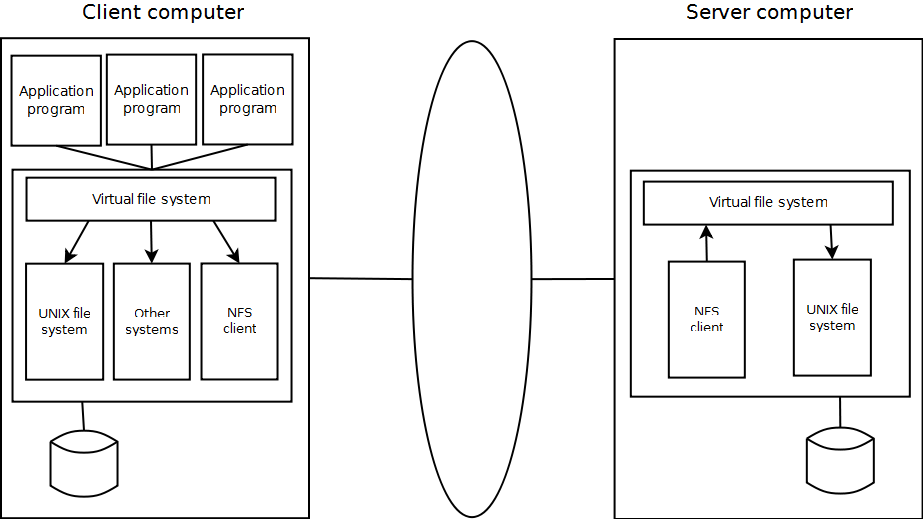
\includegraphics[width=0.7\textwidth]{img/nfs}
	\end{center}
	\caption{Sun NFS architecture.}
	\label{fig:nfs}
\end{figure}



\subsubsection{Virtual file system}

Sun NFS tries to achieve access transparency through a \emph{virtual file system (VFS)} that provides an abstraction layer on top of local and remote files. \textbf{Figure 2} illustrates the VFS layer providing access transparency for client applications [1].

The VFS is part of the UNIX kernel to manage local file identifiers and remote file identifiers, called \emph{file handles}. A file handle is a combination of the filesystem identifier, the i-node number and the i-node generation number. The i-node number of a UNIX file is an identification within the system that the file is stored. The i-node generation number reflects the number of times the i-node number has been reused [1].


\subsubsection{Integration through interfaces}

The NFS client module is integrated in kernel and offers a standard UNIX interface. This has several advantages [2]:
\begin{itemize}
	\item No client recompilation/reloading;
	\item Single client module for all user level processes;
	\item Encryption at kernel level.
\end{itemize}

Server integration is mainly implemented for performance reasons.

In the model depicted in \textbf{figure 2} is connected to the VFS in both client and server. Communication between client and server occurs through the interface and NFS protocol.


\subsubsection{Mounting service}

The mount service is a process that runs on the NFS server. The file \emph{/etc/exports} contains the names of the local filesystems that are avilable for remote mounting. Access lists determine which hosts are permitted to mount which filesystems. Users can mount any subtree of the filesystems they have access to, based on a chosen directory [1].

Remote filesystems may either be hard-mounted or soft-mounted in a client computer [1,2]:
\begin{itemize}
	\item \textbf{Hard-mounting} : A client waits until a request for a remote file succeeds;
	\item \textbf{Soft-mounting} : Mounting failure is returned if the request does not succeed after \textit{n} retries;
\end{itemize}

At the client, multi-part file pathnames are translated to i-node references. Each i-node referencing a remote mounted directory is translated into a file handle using a separate \textit{lookup()} request to the remote server. The VFS resolves file handles to local or remote directories. Mounting performance is improved through caching [1].

An addition to this system is the automounter. The automounter dynamically mounts remote directories when an empty mount point is referenced by a client. The automounter behaves as a local NFS server for the client machine. It holds a mapping of pathnames, or \emph{mount points} against corresponding servers. As the client accesses mount points when resolving a path name, the client module invokes a \textit{lookup()} request on the local automounter. The automounter triggers a number of probe requests to the corresponding NFS servers. Finally the referenced file systems are mounted onto the mount points via a symbolic link to avoid redundant requests to automounter [2].


\subsubsection{Caching}

Caching is done both at client and server side. Caching improves the performance of NFS significantly.

\paragraph{Server caching}

The server caching system is based on standard UNIX caching. File pages, directories, and file attributes read from disk are maintained in a memory buffer cache until the buffer space is required for other pages. Requests for files that are already in the cache then don't require expensive disk access. \emph{Read ahead} anticipates future read requests by fetching nearby file pages from memory [1].

When writes are performed in this system, additional measures are needed. The system supports two modes of writing [1]:
\begin{itemize}
	\item \textbf{Write-through} : The server writes updated file pages in the server's cache to disk before sending a reply to the client. When the reply is received, the client knows the data has been written to disk;
	\item \textbf{Delayed write} : Data stored in the cache is only written to memory when a commit operation is received for the relevant file. The client knows the file is written to disk as soon as a reply is received to a commit operation request;
\end{itemize}



\paragraph{Client caching}

Caching is used to reduce the number of requests to the server. The results of the following operations are cached: \textit{read()}, \textit{write()}, \textit{getattr()}, \textit{lookup()}, and \textit{readdir()}. As a result of the delayed updates introduced by caching, different versions of the same file pages may exist simultanously at different client nodes. To solve this problem, clients use polling to check the currency of their cached data, using a timestamp based method [1].

Let \textit{Tc} be the time when the cache entry was last validated, and \textit{Tm} the time when the block was last modified at the server. A cache entry is valid at time \textit{T} if \textit{T - Tc} is less than a freshness interval \textit{t}, or if the value for \textit{Tm} recorded at the client is equal to this value recorded at the server. The value of the freshness interval \textit{t} is a tradeoff between consistency and efficiency - on a Sun Solaris client, \textit{t} lies somewhere between 3 and 30 seconds. Formally this yields to following formula:

$(T - Tc < t) \vee (Tm_{client} = Tm_{server})$ \\

The cause for recent updates not to be visible immediately at the client has two sources of delay:
\begin{itemize}
	\item The delay after the write before the updated data leaves the cache in the updating client's kernel;
	\item The window for cache validation.
\end{itemize}

When a cached page is modified, it is marked as dirty and scheduled to be flushed to the server asynchronously. Pages are flushed when a file is closed or a \textit{sync} operation occurs at the client. A \emph{bio-daemon} is used to facilitate read-ahead and delayed-write operations. A bio-daemon is notified after each read request, and it requests the transfer of the following file block from the server to the client cache. In the case of writing, the bio-daemon will send a block to the server whenever a block has been filled by a client operation [1].


\subsubsection{Access control}

The NFS server is stateless. As a result, the user's identity has to be verified against the file's access permission attributes with each request. Encryption and integration with Kerberos tries to prevent impersonation [1].







\subsection{Andrew File System}

A schematic overview of the Andrew File System is given in \textbf{figure 3}.

\begin{figure}
	\begin{center}
		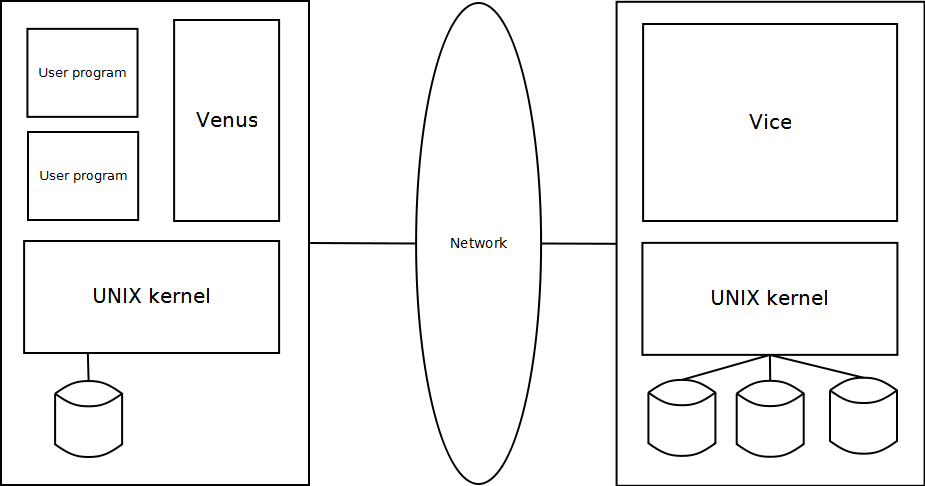
\includegraphics[width=0.7\textwidth]{img/afs}
	\end{center}
	\caption{Andrew File System architecture.}
	\label{fig:afs}
\end{figure}


The Andrew File System is characterized by two design decisions [1]:
\begin{enumerate}
	\item \textbf{Whole-file serving} : The entire file contents are transmitted to client computers by AFS servers;
	\item \textbf{Whole-file caching} : File copies at the client are stored in a cache on the local disk, i.e., the cache is permanent.
\end{enumerate}

The design strategy is based on a number of assumptions about the average and maximum file size and locality of reference to files in UNIX systems [1]:
\begin{itemize}
	\item Files are small;
	\item Read operations are much more common than write operations;
	\item Sequential access is common, random writes are rare;
	\item Most files are read and written only by one user;
	\item Files are referenced in bursts, i.e., files referenced recently are likely to be referenced again.
\end{itemize}

A scenario that illustrates the operation of AFS is as follows [1]:
\begin{enumerate}
	\item The user process in a client computer issues an \textit{open} call for a file the shared file space. There is no current copy of the file in the cache. The client sends a request to the server containing the file.
	\item The copy is stored in the local UNIX file system in the client computer. The copy is opnened and the resulting UNIX file descriptor is returned to the client.
	\item Subsequent \textit{read}, \textit{write}, etc. operations on the file by processes in the client computer are applied on the local copy.
	\item The client process issues a \textit{close} system call. If the local copy has been updated, its contents are sent back to the server. The server performs relevant updates. The client keeps its copy of the file in the cache.
\end{enumerate}

The design affects performance and the semantics of the system. Based on the previously described design characteristics, we can make the following predictions about AFS performance:
\begin{itemize}
	\item Locally cached copies remain valid for a long time if the files are updated infrequently and/or files that are updated by just a single user;
	\item The provision of sufficient cache space on a client machine ensures that files in regular use are normally retained in the cache until they are needed again;
	\item Databases do not scale well with AFS as they are updated frequently and shared by many users.
\end{itemize}



\subsubsection{Implementation}

The \emph{Vice} is server software that runs as a user-level UNIX process in each server computer. The \emph{Venus} is a user-level process that runs in the client computer. Referring to the abstract model in \textbf{figure 1}, the Venus process corresponds to the client module [1].

File in the workstations are either local or shared. Shared files are stored on servers and copies are cached in client computers. A specific subtree \textit{cmu} contains all the shared files. User directories are in the shared space, enabling file access from any workstation. One of the partitions on the local disk of each workstation is used as a cache. It is managed by the Venus component of the client [1].

Files are grouped into volumes. \emph{Fids} include the volume number of the volume containing the file, an NFS file handle identifying the file within the volume, and a \textit{uniquifier} to avoid fid reuse. The Vice servers only accept requests by the Venus in terms of fids. On the client computer pathnames are used to access files, which are then translated by the Venus component into fids [1].



\subsubsection{Caching}

When Vice supplies a copy of a file to a Venus process it also provides a callback promise. A \emph{callback promise} is a token issued by the Vice server that is the custodian of the file, guaranteeing that it will notify the Venus process when any other client modifies the file [1].

Whenever the client's Venus handles an \textit{open} operation, it checks the cache. If the required file is found in the cache, then its token is checked. The token can have two states [1]:
\begin{itemize}
	\item \textbf{Valid} : The cached copy can be opened and used without reference to Vice;
	\item \textbf{Cancelled} : A fresh copy of the file must be fetched from the Vice server. When the Venus process receives a callback, it sets the callback promise token for the relevant file to cancelled.
\end{itemize}


\paragraph{Maintaining consistency}

When a workstation is restarted after a failure or a shutdown, its Venus component cannot assume that the callback promise tokens are correct, as some callbacks may have been missed. So before a file is accessed, the Venus has to send a validation request containing the file modification timestamp to the server that is the custodian of the file. If the timestamp is current, the server responds with valid and the token is reinstated. If the timestamp shows that the file is out of date, then the server responds with cancelled and the token is set to cancelled [1].

To deal with possible communication failures, e.g., loss of callback messages, callbacks must be renewed before an \textit{open} operation if a certain amount of time has passed since the file was cached without communication from the server.

Since the majority of files are not accessed concurrently, and read operations predominate over writes in most applications, the callback mechanism results in a dramatic reduction in the number of client-server interactions [1].

The callback mechanism used in AFS requires Vice servers to maintain some state on behalf of their Venus clients, unlike NFS. To retain callback lists must be retained over server failures, they are held on the server disks and are updated using atomic operations. This design decision introduces some overhead: dealing with failures, maintaining state.


\paragraph{Update semantics}

One-copy file semantics are not practicable in large-scale systems. A strict implementation of one-copy semantics would require that the results of each write to a file are distributed to all cached copies before any further accesses can occur. The goal of the cache-consistency mechanism is to achieve an approximation of these semantics [1].

A client may open an old copy of a file after it has been updated by another client. This occurs if a callback message is lost, for example as a result of a network failure. But there is a maximum time, \textit{T}, for which a client can remain unaware of a newer version of a file. For a client \textit{C}, a file \textit{F} and corresponding custodian server \textit{S} we have the following guarantee after a successful \textit{open}:

$latest(F, S, 0) \vee (lostCallback(S, T) \wedge inCache(F) \wedge latest(F, S, T))$ \\

Here \textit{latest}(\textit{F}, \textit{S}, \textit{T}) denotes that the copy of \textit{F} seen by the client is no more than T seconds out of date, \textit{lostCallback}(\textit{S}, \textit{T}) denotes that a callback message from \textit{S} to \textit{C} has been lost at some time during the last \textit{T} seconds, and \textit{inCache}(\textit{F}) indicates that the file \textit{F} was in the cache at \textit{C} before the open operation was attempted [1].


\section*{References}

\begin{enumerate}[1]
	\item G. Coulouris, J. Dollimore, T. Kindberg and G. Blair, "Distributed Systems: Concepts and Design (5th Edition)", M. Horton, Red., Addison-Wesley, 2011, p. 1063.
	\item W. Joosen, 2013, "Distributed File Systems", iMinds-DistriNet KULeuven
\end{enumerate}
\chapter{Distributed transactions}



\section{Introduction}

Transactions are a way to describe sequences of operations by a client on a system. When these operations are invoked on different servers, the transaction becomes distributed [1]. The goal of distributed transactions is to achieve consistency of data in a distributed environment. To achieve this usually one of the servers acts as \emph{coordinator} and manages the \emph{participants} in the transaction. The coordinator keeps track of other servers, called \emph{workers}, and is responsible for final decision: when a transaction is to be finalized, agreement is needed between all servers involved to either commit or abort [2].

Transactions are said to have ACID properties [2]:
\begin{itemize}
	\item \textbf{Atomicity} : A transaction either completely succeeds or fails. In the first case the transaction will be committed and its results persisted; in the second case the transaction will have been aborted and won't have any effects.
	\item \textbf{Consistency} : A transaction moves data from one consistent state to another.
	\item \textbf{Isolation} : There is no interference from other transactions and intermediate effects are not visible to other transactions.
	\item \textbf{Durability} : Once a transaction commits, the effects of the transaction are preserved despite subsequent failures.
\end{itemize}

There are two types of transactions, based on their structure: \emph{flat transactions} and \emph{nested transactions}. In flat transactions all work is done at the same level between the start of the transaction and the commit or abort message. It is also not possible to commit or abort parts of a flat transaction.

\textbf{Table 1} gives an overview of the operations associated with flat transactions. \textbf{Figure 1} shows a general model for flat distributed transactions.

\begin{table}
	\caption{Operations in coordinator for flat transactions.}
	\label{tab:api:flattransactions}
	\begin{tabular}{p{150px} | p{250px}}
		\textbf{Operation} & \textbf{Description} \\
		\hline
		openTransaction () $\rightarrow$ trans; 		& \emph{Starts a new transaction and delivers a unique transaction identifier (TID) trans. This identifier will be used in other operations in the transaction.} \\
		closeTransaction (trans) $\rightarrow$ commit, abort; & \emph{Ends a transaction: a commit return value indicates that the transaction has committed; an abort return value indicates that it has aborted.} \\
		abortTransaction (trans); & \emph{Aborts the transaction.} \\
		join (trans, participant); & \emph{Informs a coordinator that a new participant has joined the transaction trans.} \\
		\hline
	\end{tabular}
\end{table}



\begin{figure}
	\begin{center}
		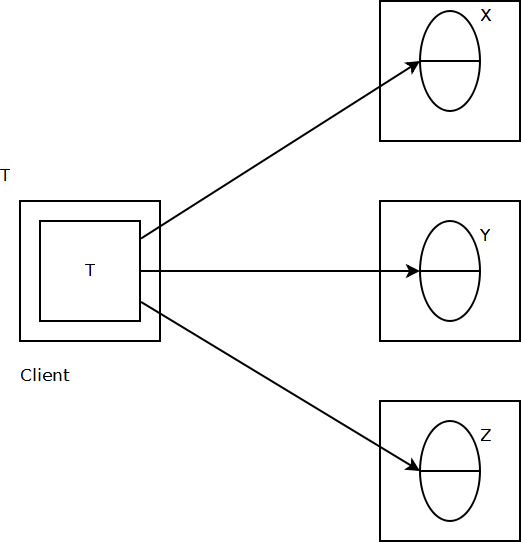
\includegraphics[width=0.4\textwidth]{img/flattransaction}
	\end{center}
	\caption{Flat transaction.}
	\label{fig:flattransaction}
\end{figure}



Nested transactions have finer grained recovery from failures as sub-transactions fail independent. Sub-transactions commit or abort independently, without effect on the outcome of other sub-transactions or enclosing transactions. The effects of sub-transactions becomes durable only when top-level transaction commits [2].

\textbf{Table 2} gives an overview of the operations associated with nested transactions. \textbf{Figure 2} depicts a general model for nested distributed transactions.

\begin{table}
	\caption{Operations in coordinator for nested transactions.}
	\label{tab:api:nestedtransactions}
	\begin{tabular}{p{150px} | p{250px}}
		\textbf{Operation} & \textbf{Description} \\
		\hline
		openSubTransaction (trans) $\rightarrow$ subTrans; 								& \emph{Opens a new subtransaction whose parent in trans and returns a unique subtransaction identifier.} \\
		getStatus (trans) $\rightarrow$ committed, aborted, provisional; 	& \emph{Asks the coordinator to report on the status of the transaction trans. Returns values representing one of the following: committed, aborted or provisional.} \\
		\hline
	\end{tabular}
\end{table}



\begin{figure}
	\begin{center}
		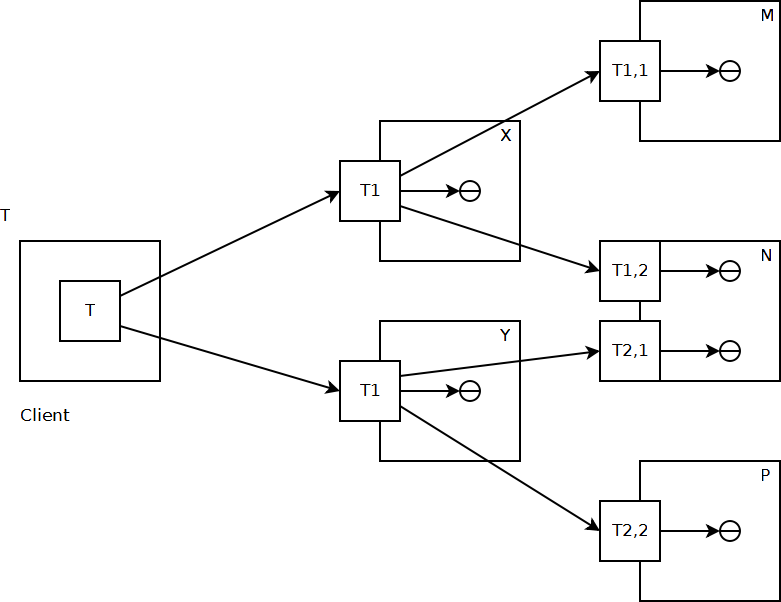
\includegraphics[width=0.6\textwidth]{img/nestedtransaction}
	\end{center}
	\caption{Nested transaction.}
	\label{fig:nestedtransaction}
\end{figure}



\section{Two-phase commit protocols}

The goal of an atomic commit protocol is to ensure that the requirements for transactions are met [1]. The protocol must work correctly, even when some servers fail messages are lost servers are temporarily unable to communicate [2].

The two-phase commit protocol consists out of a votong phase and a completion phase. The completion depends on the outcome of the voting. In the voting phase participants vote for the transaction to be committed or aborted. Once voted for commit, a participant must ensure it can actually carry out the commit. In that case the participant will remain in a \emph{prepared} state. As soon as the coordinator gives a signal that the votes where all in favour of a commit, the result transaction can be committed. In the other case, the transaction is aborted.

The protocol as given in [1] is as follows and is based on the operations listed in \textbf{table 1}; \textbf{figure 3} gives an example scenario of how the protocol is used:

\begin{itemize}
	\item 
		\textbf{Phase 1 (voting phase) :}
		\begin{enumerate}
			\item The coordinator sends a \emph{canCommit?} request to each of the participants in the transaction.
			\item When a participant receives a \emph{canCommit?} request it replies with its vote (\emph{Yes} or \emph{No}) to the coordinator. Before voting \emph{Yes}, it prepares to commit by saving objects in permanent storage. If the vote is \emph{No}, the participant aborts immediately.
		\end{enumerate}
	
	\item 
		\textbf{Phase 2 (completion according to outcome of votes) :}
		\begin{enumerate}
			\setcounter{enumi}{2}
			\item The coordinator collects the votes (including its own).
				\begin{enumerate}[a.]
					\item If there are no failures and all the votes are \emph{Yes}, the coordinator decides to commit the transaction and sends a \emph{doCommit} request to each of the participants.
					\item Otherwise, the coordinator decides to abort the transaction and sends doAbort requests to all participants that voted \emph{Yes}.
				\end{enumerate}
			\item Participants that voted \emph{Yes} are waiting for a \emph{doCommit} or \emph{doAbort} request from the coordinator. When a participant receives one of these messages it acts accordingly and, in the case of commit, makes a \emph{haveCommitted} call as confirmation to the coordinator.
		\end{enumerate}
\end{itemize}


\begin{table}
	\caption{Operations for the two-phase commit protocol.}
	\label{tab:api:twophasecommit}
	\begin{tabular}{p{150px} | p{250px}}
		\textbf{Operation} & \textbf{Description} \\
		\hline
		canCommit (trans) $\rightarrow$ Yes / No; 		& \emph{Call from coordinator to participant to ask whether it can commit a transaction. Participant replies with its vote.} \\
		doCommit (trans); 														& \emph{Call from the coordinator to participant to tell participant to commit its part of a transaction.} \\
		doAbort (trans);															& \emph{Call from coordinator to participant to tell participant to abort its part of the transaction.} \\
		haveCommitted (trans, participant); 					& \emph{Call from participant to coordinator to confirm that it has committed the transaction.} \\
		getDecision (trans) $\rightarrow$ Yes / No; 	& \emph{Call from participant to coordinator to ask for the decision on a transaction when it has voted Yes but still had no reply after some delay. Used to recover from server crash or delayed messages.} \\
		\hline
	\end{tabular}
\end{table}


\begin{figure}
	\begin{center}
		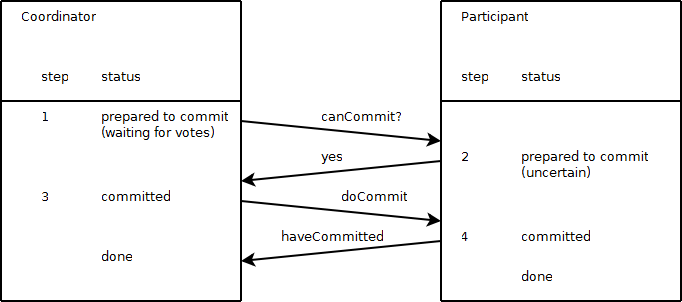
\includegraphics[width=0.6\textwidth]{img/twophasecommit}
	\end{center}
	\caption{Communication in the two-phase commit protocol.}
	\label{fig:twophasecommit}
\end{figure}




For nested transactions, when a subtransaction completes, it either to commits provisionally or aborts. The decision is made indepently. A provisional commit differs from the prepared state in that nothing is backed up in permanent storage. Once all subtransactions have completed, the ones that have been committed provisionally will try to commit their results using the two-phase commit protocol with an additional constraint: if a parent transaction has aborted, the subtransactions will abort as well. A parent transaction however, can commit even if one of its subtransactions has aborted, depending on the implementation [1]. An example of how these transactions are structured is shown in \textbf{figure 4}.

\begin{figure}
	\begin{center}
		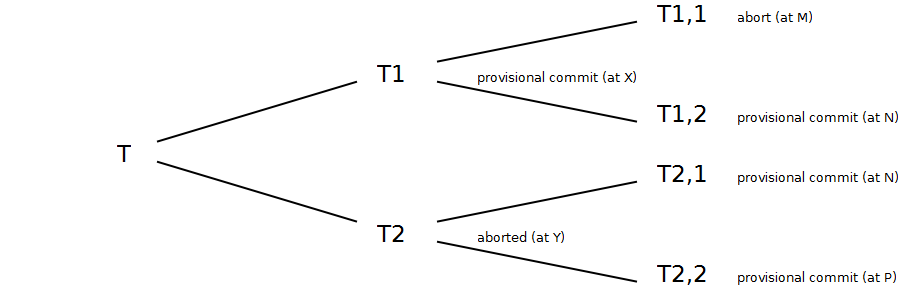
\includegraphics[width=0.8\textwidth]{img/twophasecommitnestedtransaction}
	\end{center}
	\caption{Example scenario for two-phase commit in nested transactions (based on the system depicted in figure 2).}
	\label{fig:twophasecommitnestedtransaction}
\end{figure}


There are two datastructures that are held at the coordinator: a commit list, i.e., a list of all committed (sub)transactions, and an abort list, i.e., a list of all aborted (sub)transactions [2]. The complete datastructure then consists of a list of all transactions, each with a list of their corresponding direct child transactions and commit and abort list [2].



\section{Concurrency}

Servers manage their objects and are responsible for their consistency. Concurrency control is an important aspect of transactions: transactions that access objects in a conflicting way must be handled in the same order by all servers [1].

There are a number of protocols to achieve concurrency control:
\begin{itemize}
	\item \textbf{Locking} : \emph{Locks} are used to facilitate concurrency control. They are held locally at each server. Locks are only released when a transaction has either been committed or aborted at all servers [3].
	\item \textbf{Optimistic concurrency control}
	\item \textbf{Timestamp ordering} : The ordering of transactions can be done through timestamps.
\end{itemize}

\subsection{Locking}

In nested transactions child transactions inherit locks from their parent. When a nested transaction commits, its locks are inherited by its parents, when it aborts, its locks are removed [3].

A transaction is not allowed any new locks after it has released a lock. This results in serial equivalence and requires all of a transaction's accesses to a particular data item to be serialized with respect to accesses by other transactions, and all pairs of conflicting operations of two transactions to be executed in the same order [2]. This results in the \emph{two-phase locking} protocol, consisting of the following two steps:
\begin{enumerate}
	\item \textbf{Growing phase} : New locks can be acquired;
	\item \textbf{Shrinking phase} : No new locks and release of locks.
\end{enumerate}
By releasing locks only at commit or abort, intermediate results can be hidden [2].




\subsection{Optimistic concurrency control}

\subsection{Timestamp ordering}

In the case of distributed transactions, the coordinators must issue globally unique timestamps, which they subsequently correspond to each other. To achieve the same ordering at all severs, the coordinators agree to the ordering of their timestamps [1].




\section{Distributed deadlocks}

To detect deadlocks a wait-for graph can be created. If there exists a cycle in the wait-for graph, a deadlock has occurred. A wait-for graph a directed graph G(\textit{V}, \textit{E}), where the vertices \textit{V} represent transactions and objects, and the edges \textit{E} represent either an object held by a transaction or a transaction waiting for an object [1]. An example is shown in \textbf{figure}. A \emph{distributed deadlock} occurs when there is a cycle in the global \emph{wait-for graph}, as opposed to the local wait-for graph at the server/clients themselves.

A particular problem that occurs in distributed deadlock detection are \emph{phantom deadlocks}. This is a scenario where a deadlock is detected in an outdated wait-for graph. As it may take some time to construct the full graph, a waiting transaction may have already been aborted causing a resource to be no longer required by the corresponding process. Hence, other transactions may be aborted unnecessarily to resolve the phantom deadlock [1]. If transactions are using two-phase locks, they cannot release objects and then obtain more objects, and phantom deadlock cycles cannot occur in the way suggested here [1].

There exist centralized and decentralized approaches to construct a global wait-for graph. In the following paragraphs we will discuss an example of both.


\subsection{Centralized deadlock detection}

In centralized deadlock detection one server has the responsibility for detecting deadlocks. Each time after a certain time interval, each server sends the lastest copy of its local wait-for graph to this global deadlock detector. When a deadlock is detected, it makes a decision on how to resolve it and notifies the servers which transactions to abort [1].

This kind of deadlock detection has some obvious disadvantages [1]:
\begin{itemize}
	\item Poor availability;
	\item Lack of fault tolerance;
	\item Poor scalability.
\end{itemize}


\subsection{Distributed deadlock detection: the edge-chasing algorithm}

A distributed approach to deadlock detection uses a technique called \emph{edge chasing} or \emph{path pushing}. Here, the global wait-for graph is not constructed, but each of the servers involved has knowledge about some of its edges. The servers attempt to find cycles by forwarding messages called \emph{probes}, which follow the edges of the graph throughout the distributed system. A probe message consists of transaction wait-for relationships representing a path in the global wait-for graph [1].

Edge-chasing algorithms have three steps [1]:
\begin{enumerate}
	\item \textbf{Initiation} : When a server notes that a transaction T starts waiting for another transaction U, where U is waiting to access an object at another server, it initiates detection by sending a probe containing the edge < T $\rightarrow$ U > to the server of the object at which transaction U is blocked. If U is sharing a lock, probes are sent to all the holders of the lock. Sometimes further transactions may start sharing the lock later on, in which case probes can be sent to them too.
	\item \textbf{Detection} : Detection consists of receiving probes and deciding whether a deadlock has occurred and whether to forward the probes. The global wait-for graph is built one edge at the time. As soon as cycle is detected, a deadlock has occurred.
	\item \textbf{Resolution} : When a cycle is detected, a transaction in the cycle is aborted to break the deadlock.
\end{enumerate}


\section*{References}

\begin{enumerate}[1]
	\item G. Coulouris, J. Dollimore, T. Kindberg and G. Blair, "Distributed Systems: Concepts and Design (5th Edition)", M. Horton, Red., Addison-Wesley, 2011, p. 1063.
	\item W. Joosen, 2013, "Distributed Systems - Transactions - I", IBBT-DistriNet, KULeuven
	\item W. Joosen, 2013, "Distributed Systems : Transactions - Part 2", IBBT-DistriNet, KULeuven
\end{enumerate}
\chapter{Replication}


\section{Definitions and models}

\emph{Replication} is "the maintenance of copies of data at multiple computers" [1]. In the context of replication data can be thought of as \emph{objects}, where each \emph{logical} object is in fact a collection of physical copies called \emph{replicas}. \emph{Replication transparency} may be included as another requirement for distributed system design. Replication helps making distributed systems more effective in three ways [1]:
\begin{enumerate}
	\item \textbf{Performance enhancement} : caching at server and client side helps resolving latency problems. Replication of immutable data is trivial, whereas data that can change over time must be kept up to date. In the latter case, the generated overhead may put a limit to the performance increase.
	\item \textbf{Increased availability} : Server failures and communication disconnections may decrease availability of resources. By keeping local copies of data, the availability of this data naturally increases.
	\item \textbf{Fault tolerance} : Maintaining correctness of replicated data is imperative for the effectiveness of the replication model.
\end{enumerate}

The model sketched in \textbf{figure 1} consists out of a number of components called \emph{replica managers} and a number of clients with a component called a \emph{front end} associated with it. Replica managers apply operations directly on the replicas, often using atomic operations. In this case the state of the replicas is a deterministic function of the initial state the collection of applied operations [1].

\begin{figure}
	\begin{center}
		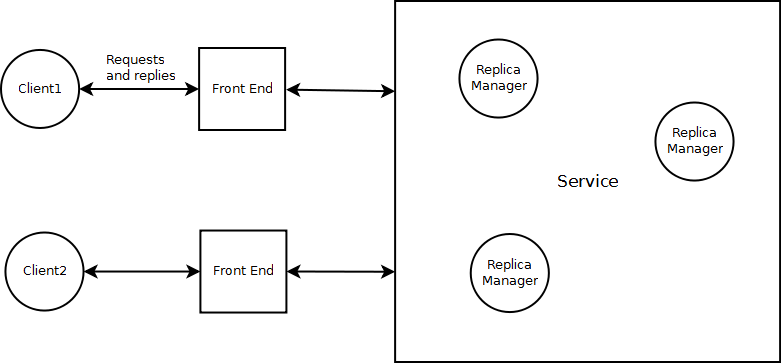
\includegraphics[width=0.7\textwidth]{img/replicationmodel}
	\end{center}
	\caption{Basic architectural model for the management of replicated data.}
	\label{fig:replicationmodel}
\end{figure}



Replica managers provide a service, i.e. access to objects, to the clients. Clients indirectly access object through the methods listed in \textbf{table 1}. The front end handles the client requests and uses messages to communicate with the replica managers. This abstraction layer ensures replication transparency at the client side [1].


\begin{table}
	\caption{Replica manager service API.}
	\label{tab:api:}
	\begin{tabular}{p{150px} | p{250px}}
		\textbf{Operation} & \textbf{Description} \\
		\hline
		readOnlyRequest (object) & \emph{Template method for an invocation by the client on an object with no updates on the object itself.} \\
		updateRequest (object) & \emph{Template method for an invocation by the client on an object, which alteres the state of the object.} \\
		\hline
	\end{tabular}
\end{table}

Coulouris et al. [1] list five phases in which the request is handles by the system:
\begin{enumerate}
	\item \textbf{Request} : The front end issues a request to one or more replica managers, either through unicast or through multicast. In the first case the replica manager will propagate the message to other replica managers.
	\item \textbf{Coordination} : Replica managers decide whether or not the request can be applied, i.e. the request will not introduce inconsistencies, and how the requests will be ordered. Possible ordering policies are for example FIFO, causal or total ordering.
	\item \textbf{Execution} : The request is executed by the replica managers.
	\item \textbf{Agreement} : The replica managers decide whether or not the commit the results of the request.
	\item \textbf{Response} : One or more replica managers communicate the result to the front end.
\end{enumerate}


\subsection{Group views}

The size of the set of replica managers may be be constant, i.e. membership is static, or vary, i.e. membership is dynamic. To manage this kind of groups, the group communication paradigm is often applied; particularly in the case of dynamic membership where the join and leave operations are concerned [1].

To manage groups, \emph{group views} are used. These are ordered lists of the current group members. Each group member has a unique process identifier. Group views are generated as members join or leave, after processes are notified of changes through view delivery. Correct view delivery requires a number of guarantees to be met [1]:
\begin{itemize}
	\item \textbf{Order} : If a processe delivers views v(g) and v'(g), then no other process will deliver v'(g) before v(g).
	\item \textbf{Integrity} : If a process delivers a view, then that process is part of the view.
	\item \textbf{Non-triviality} : A process q that is indefinitely reachable from a process p will always be in the views that p delivers.
\end{itemize}
In the case of \emph{view-synchronous group communication} additional constraints are to be met. \textbf{Figure 2} gives an overview of allowed and disallowed scenarios based on the following requirements [1]:
\begin{itemize}
	\item \textbf{Agreement} : Correct processes deliver the same sequence of views and set of messages within any given view.
	\item \textbf{Integrity} : If a correct process delivers a message m, this process will not deliver m again.
	\item \textbf{Validity} : Correct processes always deliver the messages that they send.
\end{itemize}



\begin{figure}
        \centering
        \begin{subfigure}[t]{0.4\textwidth}
                                        \centering
                                        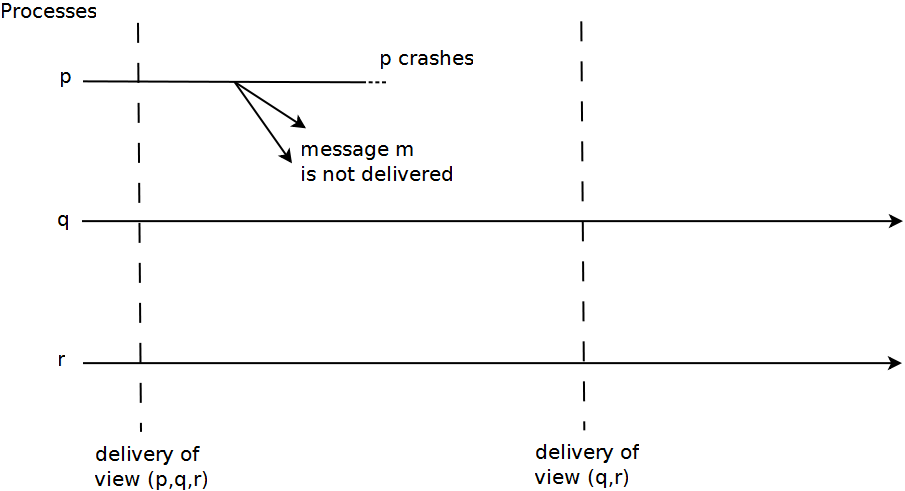
\includegraphics[width=\textwidth]{img/viewsynchronousgroupcommunication_a}
                                        \caption{Allowed case where the messages are not delivered and process p crashes.}
                                        \label{figure:viewsynchronousgroupcommunication:a}
        \end{subfigure}%
        ~
        \begin{subfigure}[t]{0.4\textwidth}
                                        \centering
                                        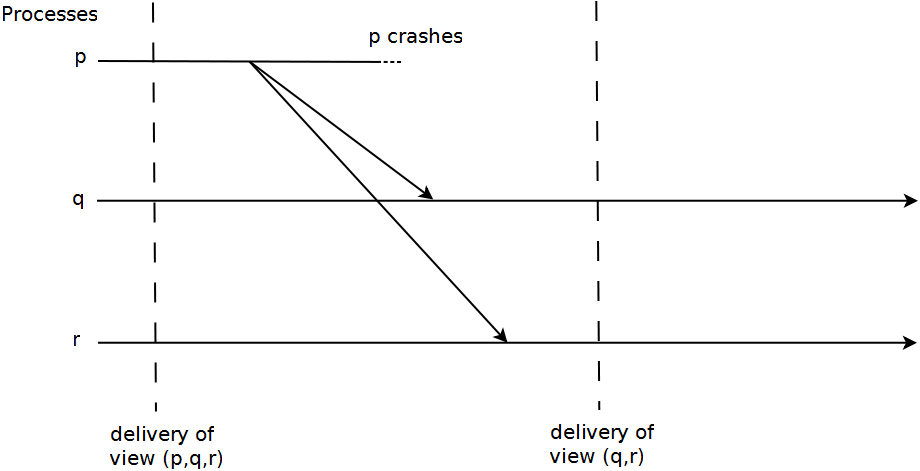
\includegraphics[width=\textwidth]{img/viewsynchronousgroupcommunication_b}
                                        \caption{Allowed case where the messages are delivered before the delivery of view (q,r).}
                                        \label{figure:viewsynchronousgroupcommunication:b}
        \end{subfigure}
        ~
        \begin{subfigure}[t]{0.4\textwidth}
                                        \centering
                                        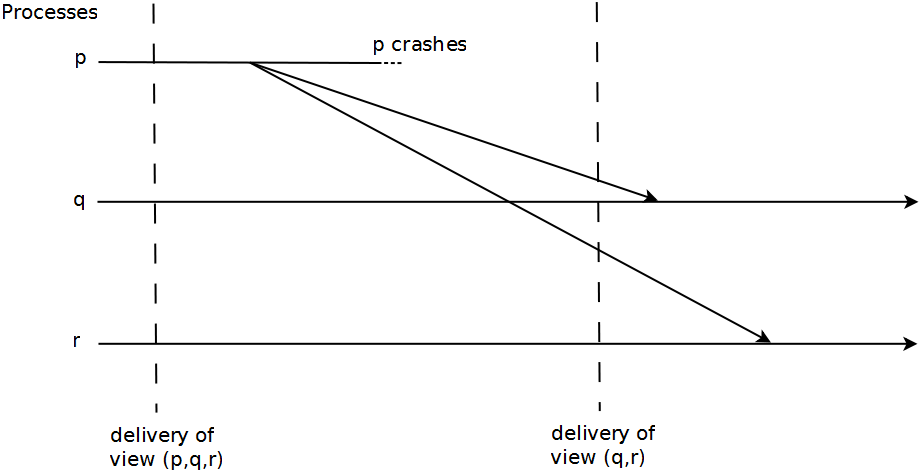
\includegraphics[width=\textwidth]{img/viewsynchronousgroupcommunication_c}
                                        \caption{Disallowed case where the messages are delivered after the delivery of view (q,r) which does not contain the crashed process p.}
                                        \label{figure:viewsynchronousgroupcommunication:c}
        \end{subfigure}
        ~
        \begin{subfigure}[t]{0.4\textwidth}
                                        \centering
                                        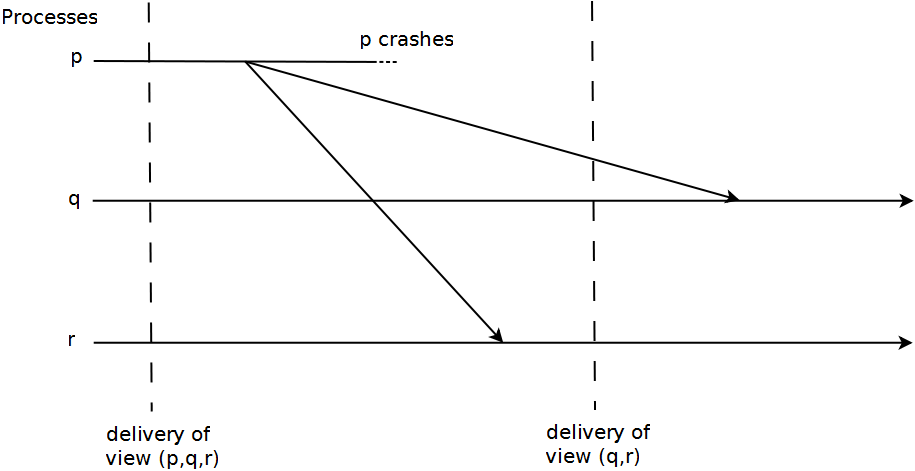
\includegraphics[width=\textwidth]{img/viewsynchronousgroupcommunication_d}
                                        \caption{Disallowed case where the messages are delivered in an incorrect order with regard to view delivery of (q,r).}
                                        \label{figure:viewsynchronousgroupcommunication:d}
        \end{subfigure}
        \caption{A selection of the screens used in the user study with paper prototype.}%
        \label{figure:viewsynchronousgroupcommunication}%
\end{figure}


View-synchronous group communication can be used to perform state transfer from the current group to new members. To ensure that the transferred state is not corrupt, the execution is usually temporary suspended. When the transfer is complete, the coordinator sends a message to the group members to continue.

The goal of group views is to increase fault-tolerance and transparency. As members crash or become unreachable, they are marked "suspicious" and may be excluded from the group by the membership service. This introduces a design challenge, as when excluding processes that are falsely excluded, resources and processing power may be (temporary) lost [1].

Another design decision has to be made in how to handle network partitions. Two general approaches exist: either the group is reduced, keeping only the primary-partition, or the group is partitionable into subgroups that can continue working independently [1].



\subsection{Fault tolerance}

The goal of fault tolerant systems is to "provide a service that is correct despite up to f process failures" [1]. This can be achieved by replicating data and functionality at replica managers. Correctness of replicated objects is subject to a number of criteria, which can vary in strictness.

\emph{Linearizability} is a strong correctness requirement. Consider a sequence of operation invocations and responses, called a \emph{history}, $o_{2,0}$, $o_{2,1}$, $o_{1,0}$, $o_{2,2}$, $o_{1,1}$, $o_{1,2}$, ..., where \emph{i} represents a client performing an operation \emph{j} for an operation $o_{i,j}$. \textbf{Figure 3 (a)} shows an overview of this setup. "A replicated shared object is linearizable if for any execution there is some interleaving of the series of operations issued by all clients that satisfies the following criteria" [1] :
\begin{itemize}
	\item The interleaved sequence of operations meets the specification of a (single) correct copy of the objects.
	\item The order of operations in the interleaving is consistent with the real times at which the operations occurred in the actual execution.
\end{itemize}
\textbf{Figure 3 (b)} shows how the operations in the history can be re-ordered. If there exists an ordering for which the previous conditions are met, the system is linearizable. In \textbf{figure 3 (c)} the new ordering did not meet the requirement.


\begin{figure}
        \centering
        \begin{subfigure}[t]{0.3\textwidth}
                                        \centering
                                        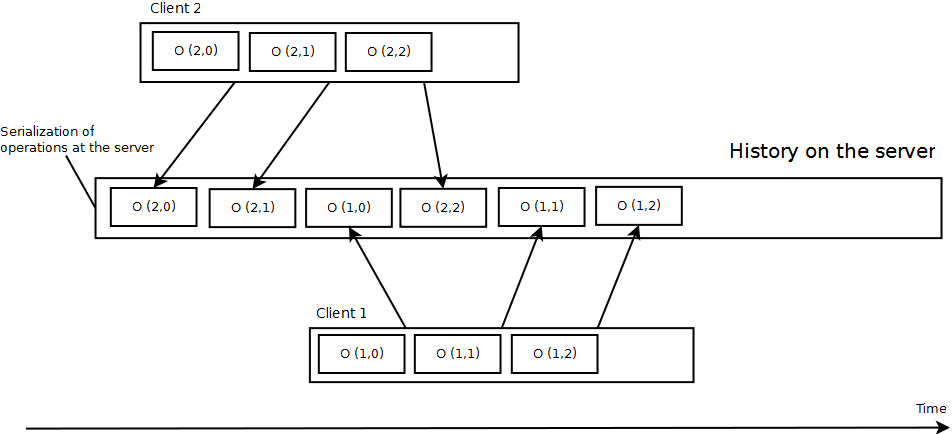
\includegraphics[width=\textwidth]{img/linearizability_1}
                                        \caption{Two clients executing operations on a replicated object managed by a server. The operations are serialized by the server into a certain sequence.}
                                        \label{figure:linearizability:a}
        \end{subfigure}%
        ~
        \begin{subfigure}[t]{0.3\textwidth}
                                        \centering
                                        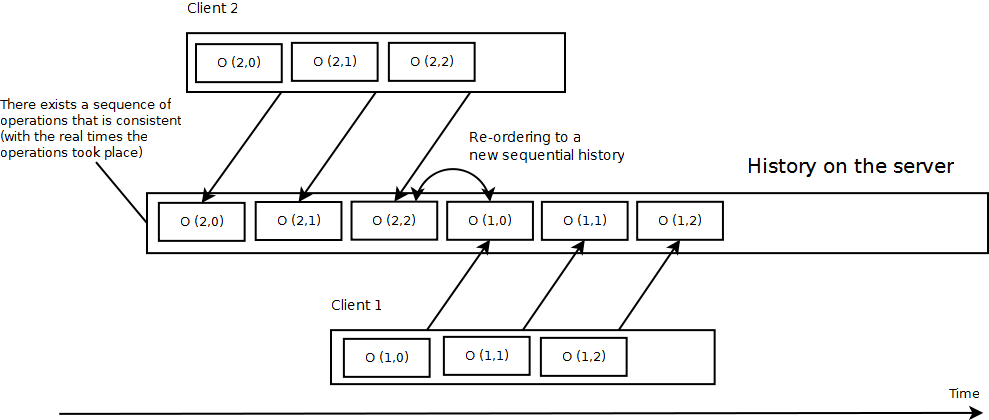
\includegraphics[width=\textwidth]{img/linearizability_2}
                                        \caption{The order of operations can be altered (serializibility) to obtain a new sequence that is consistent with the real times at which the operations occurred in the actual execution.}
                                        \label{figure:linearizability:b}
        \end{subfigure}
        ~
        \begin{subfigure}[t]{0.3\textwidth}
                                        \centering
                                        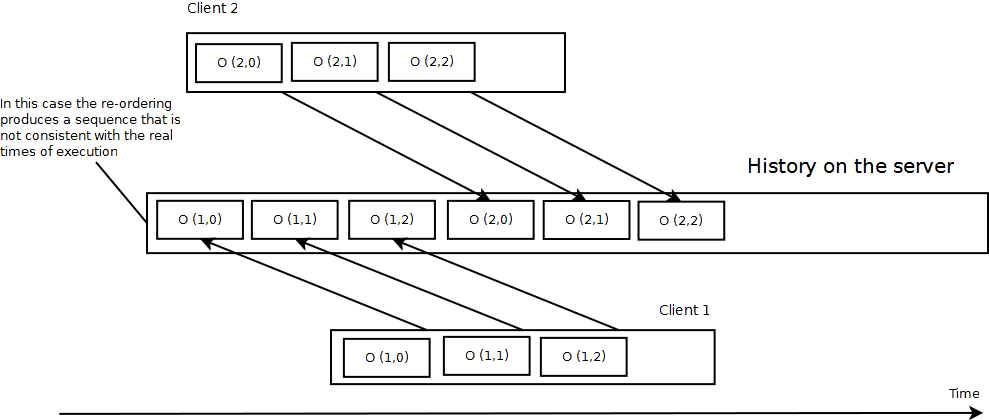
\includegraphics[width=\textwidth]{img/linearizability_3}
                                        \caption{The new sequence that is consistent not with the real times at which the operations occurred in the actual execution.}
                                        \label{figure:linearizability:c}
        \end{subfigure}
        \caption{}
        \label{figure:linearizability}
\end{figure}


\emph{Sequential consistency} is an example of a weak correctness critrium. The requirements for sequential consistency are the following:
\begin{itemize}
	\item The interleaved sequence of operations meets the specification of a (single) correct copy of the objects.
	\item The order of operations in the interleaving is consistent with the program order in which each individual client executed them.
\end{itemize}
As a result, the situation in \textbf{figure 3 (c)} is valid under a sequential consistency requirement. The absolute times are not important top obtain sequential consistency, just the order of events corresponding the clients seperately. It should be clear that sequential consistency is a much weaker constraint than linearizability. There may still be inconsistencies in the overal history, despite equential consistency. For example [2] when two clients try to lock an object, one lock will be successful and the other won't. In the case of sequential consistency, it is possible that the negative response is ordered before the successful response, which is not consistent with the sequential definition of the object, i.e. the first one to lock should have gotten a response of success.


\subsubsection{Passive replication}

The model for \emph{passive replication}, the so-called \emph{primary backup model of replication for fault tolerance}, consists out of primary replica manager and a collection of secondary replica managers or "backups". All operations are processed by the primary replica manager and afterwards changes are propagated to the backups. If the primary replica manager should fail, one of the backups is promoted to primary replica manager [1]. \textbf{Figure 4} shows an overview of this model.


\begin{figure}
	\begin{center}
		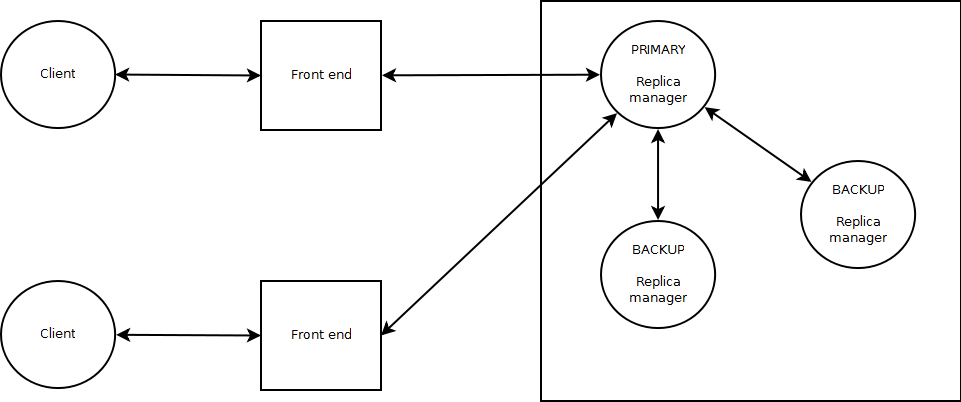
\includegraphics[width=0.7\textwidth]{img/passivereplication}
	\end{center}
	\caption{Passive replication model for fault tolerance.}
	\label{fig:passivereplication}
\end{figure}

The following steps occur when an operation is performed by a client [1]:
\begin{enumerate}
	\item \textbf{Request} : The front end issues the request, containing a unique identifier, to the primary replica manager.
	\item \textbf{Coordination} : The primary takes each request anatomically, in the order in which it receives it. It checks the unique identifier, in case it has already executed the request, and if so, it simply resends the response.
	\item \textbf{Execution} : The primary executes the request and stores the response.
	\item \textbf{Agreement} : If the request is an update, then the primary sends the updated state, the response and the unique identifier to all the backups. The backups send an acknowledgement.
	\item \textbf{Response} : The primary responds to the front end, which hands the response back to the client.
\end{enumerate}

The primary sequences all the operations upon the shared objects, so as long as the primary is correct, the system is linearizable. In the case that the primary fails, however, to ensure linearizability, the primary replica manager has to be replaced by a unique backup, and the remaining replica managers agree which operations had been performed when the replacement primary takes over. This will be the case if the replica managers apply view-synchronous group communication to send updates to the backups [1].



\subsubsection{Active replication}

In \emph{active replication} the replica managers are state machines with equivalent status and organized as a group. The front end multicasts requests to the group. Within the group each manager processes the requests independently in the same manner and reply individually to the front end [1]. \textbf{Figure 5} shows the model for active replication.

\begin{figure}
	\begin{center}
		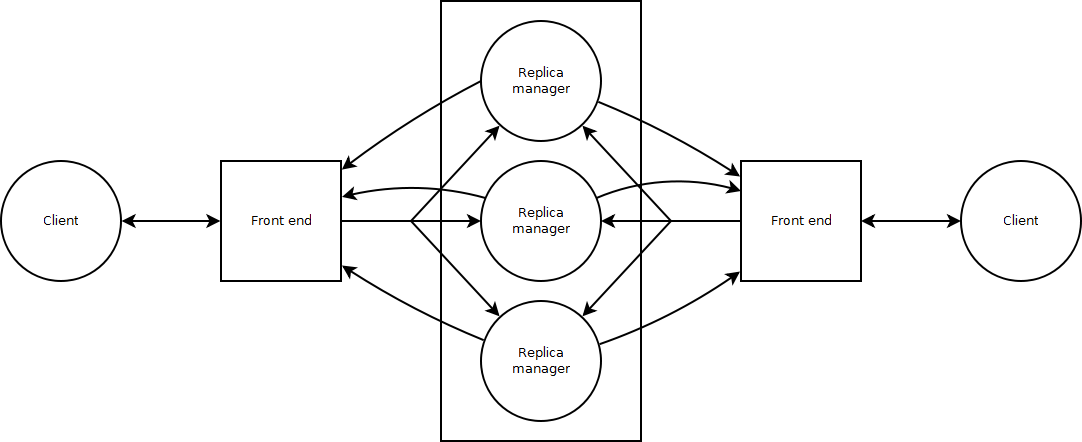
\includegraphics[width=0.7\textwidth]{img/activereplication}
	\end{center}
	\caption{Active replication model for fault tolerance.}
	\label{fig:activereplication}
\end{figure}


The following steps occur when an operation is performed by a client [1]:
\begin{enumerate}
	\item \textbf{Request} : The front end attaches a unique identifier to the request and multicasts it to the group of replica managers, using a totally ordered, reliable multicast primitive. The front end is assumed to fail by crashing at worst.It does not issues the next request until it has received a response.
	\item \textbf{Coordination} : The group communication system delivers the request to every correct replica manager in the same (total) order.
	\item \textbf{Execution} : Every replica manager executes the request. Since they are state machines and since requests are delivered in the same total order, correct replica managers all process the request identically. The response contains the client's unique request identifier.
	\item \textbf{Agreement} : No agreement phase is needed, because of multicast delivery semantics.
	\item \textbf{Response} : Each replica manager sends its response to the front end. The number of replies that the front end collects depends upon the failure assumptions and the multicast algorithm.
\end{enumerate}

The system is sequentially consistent, but does not achieve linearizability since the total ordering is not necessarily the same as the real-time order in which the clients made their requests [1].

Crashes of replica managers have little impact on the performance in active replication, as the remaining replica managers continue to work as usual. Because the front end can compare the replies it receives, the system is less prone to Bynzantine failures [1].


\subsubsection{Comparison: active and passive replication}


\begin{table}
	\caption{Comparison between passive and active replication.}
	\label{tab:compare:replication:faulttolerance}
	\begin{tabular}{p{80px} | p{155px} | p{155px}}
															& \textbf{Passive} & \textbf{Active} \\
		\hline
		\textbf{Correctness} 			& Support for linearizability. & Support up to sequential consistency. \\
		\textbf{Fault tolerance} 	& The system requires f+1 replica managers to survive up to f process crashes. & For f Byzantine failures, the system requires 2f+1 replica managers to ensure that the system continues to function correctly. This is because the front collects f+1 replies before passing on the results to the client. \\
		\textbf{Efficiency} 			& View-synchronous group communication is required to support linearizability, but introduces a significant overhead. In a variation where read requests are handled by backups to improve performance, the system looses its linearizability property, but maintains sequential consistency. & As managers work independently within te group, crashes have no impact on efficiency. The group communication is relatively cheap as no view-synchronous communication is required. \\
		\hline
	\end{tabular}
\end{table}




\section{Highly available services: examples of systems using replication}

\subsection{The Coda file system}


The Coda file system is based on the Andrew File System (AFS). It was developed to address additional requirements for file systems, in particular to provide high availability in presence of disconnected operations. Of course, Coda retains the original goals of AFS with regard to scalability and the emulation of UNIX file semantics. Coda tries to meet the following three additional requirements under the general heading of constant data availability [1,2]:

\begin{enumerate}
	\item \textbf{Performance} : In large-scale distributed systems this availability requirement becomes more important, as the limited form of replication offered by AFS on read-only volumes doesn't scale well for accessing widely shared files.
	\item \textbf{Fault tolerance} : The availability of AFS services was to be improved as failures (or scheduled interruptions) of servers and network components could make these services inaccessible for significant periods of time.
	\item \textbf{Disconnect operations due to mobility} : Finally, mobile computers disconnect and reconnect frequently leading to an availability requirement of files the user may need despite being disconnected [1].
\end{enumerate}

The design of Coda relies on the replication of file volumes to achieve a higher throughput of file access operations and a greater degree of fault tolerance. Coda also makes use of AFS's client caching extension [1]. Coda enhances availability both by [1]:
\begin{itemize}
	\item Replication of files across servers. The advantages of replicating file volumes on multiple servers are [1]:
		\begin{itemize}
			\item As long as at least one replica is accessible the client can access the files in that replicated volume.
			\item System performance can be improved by sharing some of the load, i.e. client requests on replicated volumes, between the servers holding replicas.
		\end{itemize}
	
	\item The ability of clients to operate entirely out of their caches. Coda will try to predict which files will be needed by a user and cache them in case of disconnection with the network.
\end{itemize}



\subsubsection{The Coda architecture}

\paragraph{Vice (server) and Venus (client) processes}

\textbf{Figure 6} shows an overview of the Coda file system architecture. Similar to AFS, Coda runs \emph{Venus} processes at the client computers and \emph{Vice} processes at file server computers. The Vices are the replica managers, and the Venuses are a hybrid of front ends and replica managers. A Venus plays the front end's role of hiding the service implementation from local client processes, but since they manage a local cache of files they are also replica managers.

\begin{figure}
	\begin{center}
		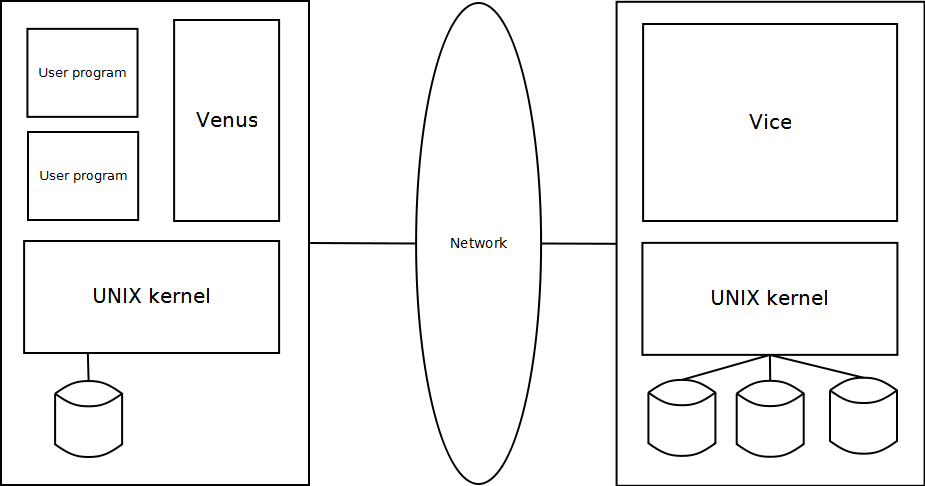
\includegraphics[width=0.7\textwidth]{img/afs}
	\end{center}
	\caption{Coda file system architecture (AFS-based).}
	\label{fig:coda}
\end{figure}



\paragraph{The volume storage group (VSG)}

A volume storage group (VSG) is the set of servers that holds replicas of a file volume. As servers become inaccessible as a result of network or server failures, the client can usually only access a subset of the VSG, known as the available volume storage group (AVSG). A disconnected operation occurs when the AVSG is empty [1].



\subsubsection{Replication and consistency}

The Coda servers are the focal point to provide quality of service, as cached file copies residing on client computers are regarded as less reliable than those at the servers. These files are periodically revalidated against the version at the servers. In presence of network partitions updated files may cause conflicts with other replicas when the network is restored [1].

Coda uses an optimistic replication strategy, i.e. files can be modified in presence of network partitions or during disconnected operations.


\paragraph{Coda version vector}

Each version of a file has a \emph{Coda version vector} (CVV) containing a timestamp with one element for each server in the corresponding VSG [1]. When a modified file is closed, the Venus process sends an update message with the current CVV and the new contents for the file to the AVSG. If the CVV is greater than the one currently held at the AVSG, the new contents for the file are stored and a positive acknowledgement is returned. The Venus process then computes a new CVV with modification counts increased for the servers that responded positively to the update message and distributes the new CVV to the members of the AVSG. Note that AVSG is only a subset of the VSG, so possibly not all members will receive the new CVV [1].

The CVV can be used for resolving file conflicts as follows. For timestamps of two CVVs $v_{1}$ and $v_{2}$, there are two general cases [1]:
\begin{itemize}
	\item If the CVV at one of the sites is greater than or equal to all the corresponding CVVs at the other sites then there is no conflict.
	\item When neither $v_{1} \leq v_{2}$ nor $v{1} \geq v_{2}$ holds for two CVVs then there is a conflict: each replica reflects at least one update that the other does not reflect. Coda does not, in general, resolve conflicts automatically. The file is marked as \emph{inoperable} and the owner of the file is informed of the conflict.
\end{itemize}



\paragraph{Accessing replicas and update semantics}

AFS's original \emph{callback promise} mechanism, is extended and depends on an additional mechanism for the distribution of updates to each replica. The strategy used on open and close on the replicas is a variant of the \emph{read-one/write-all} approach [1]. \textbf{Table 3} lists the open and close operation specifics.


\begin{table}
	\caption{File open and close operation in Coda.}
	\label{tab:api:coda}
	\begin{tabular}{p{150px} | p{250px}}
		\textbf{Operation} & \textbf{Description} \\
		\hline
		open 	& This operation consists of the following steps. If a copy of the file is not present in the local cache:
				\begin{enumerate}
					\item The client choses a preferred server from the AVSG for the file.
					\item The client requests a copy of the file attributes and contents from the preferred server.
					\item The client checks with all the other members of the AVSG to verify that the copy is the latest available version. If not, a member of the AVSG with the latest version is made the preferred site, the file contents are refetched and the members of the AVSG are notified that some members have stale replicas.
					\item When the fetch has been completed, a callback promise is established at the preferred server.
				\end{enumerate} \\
		close & On close, copies of modified files are broadcast in parallel to all of the servers in the AVSG using \emph{multicast remote procedure calling protocol}. This has two notable effects:
				\begin{enumerate}
					\item It maximizes the \textit{probability} that every replication site for a file has the current version at all times. It doesn't guarantee it, because the AVSG does not necessarily include all the members of the VSG.
					\item It minimizes the server load by giving clients the responsibility for propagating changes to the replication sites in the normal case.
				\end{enumerate} \\
		\hline
	\end{tabular}
\end{table}



The update semantics for Coda are a little different to those in AFS. The single server \textit{S} referred to in the currency guarantees for AFS is replaced by a set of servers \textit{S}, i.e. the VSG for a file \textit{F} and the client \textit{C} can access a subset of servers \textit{s}, i.e., the AVSG for that file seen by \textit{C}. \textit{T} is again the maximum time that for which a client can remain unaware of an update elsewhere to the cached file [1]. In addition the following predicates are used:
\begin{itemize}
	\item $latest(F, s, T)$ : The current value of \textit{F} at \textit{C} was the latest across all the servers in s at some instant in the last \textit{T} seconds and that there were no conflicts among the copies of \textit{F} at that instant;
	\item $lostCallback(s, T)$ : A callback was sent by some member of \textit{s} in the last \textit{T} seconds and was not received at \textit{C};
	\item $conflict(F,s)$ : The values of \textit{F} at some servers in \textit{s} are currently in conflict.
\end{itemize}


The currency guarantees are then summarized as follows [1]. In each definition except the last there are two cases [1]:
\begin{enumerate}
	\item $s \neq \emptyset$ : The AVSG is not empty, i.e., the client is not disconnected.
	\item $s = \emptyset$ : The disconnected operation.
\end{enumerate}

\textbf{After succesfull open} : The guarantee offered by a successful open is that either that the most recent copy of \textit{F} is provided from the current AVSG, or a locally cached copy of \textit{F} is used if one is available, if no server is accessible:

$(s \neq \emptyset \wedge (latest(F, s, 0) \vee (latest(F, s, T) \wedge lostCallback(s, T) \vee inCache(F))))$ \\
$\vee$ \\
$(s = \emptyset \wedge inCache(F))$ \\

\textbf{After failed open :}

$(s \neq \emptyset \wedge conflict(F, s)) \vee (s = \emptyset \wedge \neg inCache(F))$ \\

\textbf{After succesfull close} : A successful close guarantees that the file has been propagated to the currently accessible set of servers, or, if no server is available, that the file has been marked for propagation at the earliest opportunity.

$(s \neq \emptyset \wedge updated(F, s)) \vee (s = \emptyset)$ \\

\textbf{After failed close :}

$(s \neq \emptyset \wedge conflict(F, s))$ \\








\subsubsection{Caching}


\paragraph{Cache coherence}

The Coda currency guarantees stated earlier mean that the Venus process at each client must detect the following events within \textit{T} seconds of their occurrence [1]:
\begin{itemize}
	\item \textbf{AVSG size changes} : Enlargement of an AVSG (due to the accessibility of a previously inaccessible server), or shrinking of an AVSG (due to a server becoming inaccessible);
	\item \textbf{Callback event loss} : Since maintaining callback state in all the members of an AVSG would be expensive, the callback promise is maintained only at the preferred server. However, the preferred server for one client need not be in the AVSG of another client. If this is the case, an update by the second client will not cause a callback to the first client.
\end{itemize}


\subparagraph{AVSG size changes}

Venus (client) sends a probe message to all the servers in VSGs of the files that it has in its cache every \textit{T} seconds. Responses will be received only from accessible servers. The following cases can be distinguished with regard to callback reponses:
\begin{itemize}
	\item \textbf{Venus receives a response from a server that was previously inaccessible} : Venus enlarges the corresponding AVSG. As the cached copy may no longer be the latest version available, Venus will also drop the callback promises on any files that it holds from the relevant volume.
	\item \textbf{Venus fails to receive a response from a previously accessible server} : Venus shrinks the corresponding AVSG. Unless the preferred server is lost, no callback changes are required.
	\item \textbf{The preferred server is lost} : All callback promises from that server must be dropped.
	\item \textbf{A response indicates that a callback message was sent but not received} : The callback promise on the corresponding file is dropped.
\end{itemize}


\subparagraph{Disjunct AVSGs}

Venus is sent a \emph{volume version vector} (volume CVV) in response to each probe message, containing a summary of the CVVs for all of the files in the volume. If Venus detects any mismatch between the volume CVVs, then some members of the AVSG must have some file versions that are not up-to-date. Although the outdated files may not be the ones that are in its local cache, Venus makes a pessimistic assumption and drops the callback promises on all of the files that it holds from the relevant volume [1].


\paragraph{Cache miss and disconnected operation}

In disconnected operation (when none of the servers for a volume can be accessed by the client) a cache miss prevents further progress and the computation is suspended until the connection is resumed or the user aborts the process. It is therefore important to load the cache before disconnected operation commences so that cache misses can be avoided [1].

\subparagraph{Selecting files to retain in the cache}

If a client is disconnected for an extended period of time, it is likely that files or directories will be referenced that are not in the cache. To alleviate this problem Coda allows users to specify a prioritized list of files and directories that Venus should strive to retain in the cache. Objects at the highest level are identified as \emph{sticky} and these must be retained in the cache at all times. If the local disk is large enough to accommodate all of them, the user is assured that they will remain accessible [1].

\subparagraph{Reintegration after disconnect operation}

When disconnected operation ends, a process of reintegration begins. For each cached file or directory that has been modified, created or deleted during disconnected operation, Venus executes a sequence of update operations to make the AVSG replicas identical to the cached copy. Reintegration proceeds top-down from the root of each cached volume [1].




\subsection{Gossip framework}

The goal of the Gossip framework is implementing highly available services by replicate data close to points where groups of clients need it [3]. Gossip is not fault tolerant. A framework implies that it is configurable with multiple degrees of freedom. The consequence of this is that it can be used for a variety of applications [3].

\begin{figure}
	\begin{center}
		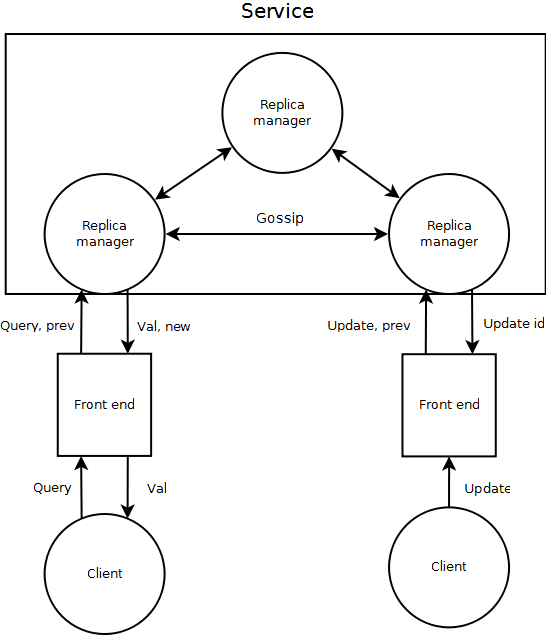
\includegraphics[width=0.6\textwidth]{img/gossiparchitecture}
	\end{center}
	\caption{The Gossip framework architecture.}
	\label{fig:gossiparchitecture}
\end{figure}


The front end sends operations to any RM that is available and has a reasonable response time. There are two types of operations [3]:
\begin{itemize}
	\item \textbf{Queries} : Read-only operations;
	\item \textbf{Updates} : Change state
\end{itemize}


\subsection{Bayou}

The goals of the Bayou model are data replication for high availability, but with weaker guarantees than sequential consistency, and coping with variable connectivity [3].




\section*{References}

\begin{enumerate}[1]
	\item G. Coulouris, J. Dollimore, T. Kindberg and G. Blair, "Distributed Systems: Concepts and Design (5th Edition)", M. Horton, Red., Addison-Wesley, 2011, p. 1063.
	\item Wikipedia, 2013, "Linearizability | Wikipedia", online, available at:  http://en.wikipedia.org/wiki/Linearizability
	\item W. Joosen, 2013, "Distributed Systems: Replicated Data - Part 1",  iMinds-DistriNet KULeuven
\end{enumerate}


\chapter{Cloud computing}


\section{What is cloud computing?}



\subsection{Characteristics}

Characteristics [2]:

\begin{itemize}
	\item \textbf{On-demand self-service} : A consumer can unilaterally provision computing capabilities, such as server time and network storage, as needed automatically without requiring human interaction with each service provider;
	\item \textbf{Broad network access} : Capabilities are available over the network and accessed through standard mechanisms that promote use by heterogeneous thin or thick client platforms, e.g., mobile phones, tablets, laptops, and workstations;
	\item \textbf{Resource pooling} : The provider's computing resources are pooled to serve multiple consumers using a multi-tenant model, with different physical and virtual resources dynamically assigned and reassigned according to consumer demand. There is a sense of location independence in that the customer generally has no control or knowledge over the exact location of the provided resources but may be able to specify location at a higher level of abstraction, e.g., country, state, or datacenter. Examples of resources include storage, processing, memory, and network bandwidth;
	\item \textbf{Rapid elasticity} : Capabilities can be elastically provisioned and released, in some cases automatically, to scale rapidly outward and inward commensurate with demand. To the consumer, the capabilities available for provisioning often appear to be unlimited and can be appropriated in any quantity at any time;
	\item \textbf{Measured service} : Cloud systems automatically control and optimize resource use by leveraging a metering capability at some level of abstraction appropriate to the type of service (e.g., storage, processing, bandwidth, and active user accounts). Resource usage can be monitored, controlled, and reported, providing transparency for both the provider and consumer of the utilized service;
\end{itemize}



Outsourcing requires trust from clients.


A number of advantages are associated with cloud computing [2]:
\begin{itemize}
	\item Accelerated deployment of new applications without consuming enterprise's existing IT resources;
	\item Reduced capital requirements for up-front IT investments;
	\item Flexibility to meet sudden changes in demand peaks and troughs;
	\item Capability to match current and future demand;
	\item Significant cost savings through centralization when scale of enterprise IT resources << cloud provider;
	\item Data sharing and collaboration for multi-party processes. More economical and faster to deploy centrally;
\end{itemize}






\subsection{Business models}

Cloudcomputing is typically a pay per use model for on-demand, convenient access to shared pool of computing resources, e.g., storage, CPU, network, and applications. There are three basic types of services in the cloud computing model [2]:
\begin{enumerate}
	\item \textbf{Infrastructure as a service (IaaS)} : virtual machine with processing, storage and networking;
	\item \textbf{Platform as a service (PaaS)} : development platform and associated tools, e.g., PHP, .NET, Java;
	\item \textbf{Software as a service (SaaS)} : Zero-install, online applications, e.g., CRM, document processing platforms, application specific record management etc.;
\end{enumerate}


\subsubsection{Infrastructure as a Service (IaaS)}

"The capability provided to the consumer is to provision processing, storage, networks, and other fundamental computing resources where the consumer is able to deploy and run arbitrary software, which can include operating systems and applications. The consumer does not manage or control the underlying cloud infrastructure but has control over operating systems, storage, and deployed applications; and possibly limited control of select networking components (e.g., host firewalls)." [3]


\subsubsection{Platform as a Service PaaS}

"A cloud service model that provides the consumer the capability to deployonto the cloud infrastructure consumer-created or acquired applicationscreated using programming languages, libraries, services, and tools supported by the provider.1The consumer does not manage or control the underlying cloud infrastructureincluding network, servers, operating systems, or storage, but has control over the deployed applications and possibly configuration settings for the application-hosting environment." [3]



\subsubsection{Software as a Service SaaS}

"The capability provided to the consumer is to use the provider's applications running on a cloud infrastructure(*). The applications are accessible from various client devices through either a thin client interface, such as a web browser (e.g., web-based email), or a program interface. The consumer does not manage or control the underlying cloud infrastructure including network, servers, operating systems, storage, or even individual application capabilities, with the possible exception of limited user-specific application configuration settings." [3]

\subsection{Value levels of cloud computing}

In [4] three value levels of cloud computing are discussed:
\begin{itemize}
	\item \textbf{Utility level} : Enterprises can benefit from lower costs and higher service levels through the availability of elastic computing resources and pay-per-use models;
	\item \textbf{Process transformation level} : Enterprises can introduce new and improved business processes by leveraging the common and scalable assets and collaborative potential of cloud computing;
	\item \textbf{Business model innovation level} : New business models can be created by linking, sharing and combining resources using cloud computing in an entire business ecosystem;
\end{itemize}



%\section{Technologies}
%
%Cloud computing involves a wide range of possible implementations and techniques; some of these are discussed in the following paragraphs.
%
%Centralized Approaches to online social networking
%
%The Need for Scalability
%Ultra large scalability of systems.
%Highly distributed content production and querying.
%Many users:
%- Business queries.
%- End-user actions.
%
%as system complexity increases, our ability to reason about that system decreases => increase the granularity at which we reason, to minimize complexity.
%
%
%New Communication Paradigms
	%- Protocol Buffers (PB)
	%- Publish-Subscribe dissemination of distributed events in real time
%
%New Models of Computation
	%- MapReduce
%
%Increasing scale further
	%- Hadoop
		%* NameNode
		%* DataNode
	%- Hive






\section*{References}

\begin{enumerate}[1]
	\item G. Coulouris, J. Dollimore, T. Kindberg and G. Blair, "Distributed Systems: Concepts and Design (5th Edition)", M. Horton, Red., Addison-Wesley, 2011, p. 1063.
	\item Wouter Joosen, 2013, "Perspectives on Cloud Computing", iMinds-DistriNet, KU Leuven
	\item P. Mell and T. Grance, 2011, "The NIST Definition of Cloud Computing", online, available at: http://csrc.nist.gov/publications/nistpubs/800-145/SP800-145.pdf
	\item D. Dean and T. Saleh, 2009: "Capturing the Value of Cloud Computing: How Enterprises Can Chart Their Course to the Next Level", BCG -http://www.bcg.be/documents/file34246.pdf
\end{enumerate}
\part{Labs}
\chapter{Java RMI}

\chapter{Java Enterprise Edition EJB}

\chapter{Google App Engine}



%%%%%%%%%%%%%%%%%%%%%%%%%%%%%%%%%%%%%%%%%%%%%%%%%%%%%%%%%%%%%
%% BIBLIOGRAPHY AND OTHER LISTS
%%%%%%%%%%%%%%%%%%%%%%%%%%%%%%%%%%%%%%%%%%%%%%%%%%%%%%%%%%%%%
%% A small distance to the other stuff in the table of contents (toc)
\addtocontents{toc}{\protect\vspace*{\baselineskip}}

%% The Bibliography
\addcontentsline{toc}{chapter}{Bibliography} %'Bibliography' into toc
\nocite{*}
\bibliographystyle{plain}
\bibliography{bib/references}

%% The List of Figures
\clearpage
\addcontentsline{toc}{chapter}{List of Figures}
\listoffigures

%% The List of Tables
\clearpage
\addcontentsline{toc}{chapter}{List of Tables}
\listoftables


%%%%%%%%%%%%%%%%%%%%%%%%%%%%%%%%%%%%%%%%%%%%%%%%%%%%%%%%%%%%%
%% APPENDICES
%%%%%%%%%%%%%%%%%%%%%%%%%%%%%%%%%%%%%%%%%%%%%%%%%%%%%%%%%%%%%
\appendix
%% ==> Write your text here or include other files.

%\input{FileName} %You need a file 'FileName.tex' for this.


\end{document}

